% !TeX spellcheck = hu_HU
\documentclass[a4paper,12pt]{article}

% Magyar nyelvi beállítások
\usepackage[utf8]{inputenc}
\usepackage[T1]{fontenc}
\usepackage[magyar]{babel}

% Linkek
\usepackage[colorlinks, allcolors=blue]{hyperref}

% Szebb betűtípus
\usepackage{lmodern}

% Matematika
\usepackage{amsmath, amssymb, amsthm, amsfonts}

% Oldalmargók
\usepackage[margin=2.5cm]{geometry}

% Színes dobozok definíciókhoz, tételekhez stb.
\usepackage{tcolorbox}
\tcbuselibrary{theorems}

%coordinate
\usepackage{tikz}

% Tételstílusok
%no counter / number within=section
\newtcbtheorem[no counter]{definition}{Def.}%
{colback=blue!5,colframe=blue!50!black,fonttitle=\bfseries}{def}

\newtcbtheorem[no counter]{theorem}{Tétel}%
{colback=green!5,colframe=green!50!black,fonttitle=\bfseries}{th}

\newtcbtheorem[no counter]{example}{Példa}%
{colback=yellow!10,colframe=yellow!50!black,fonttitle=\bfseries}{ex}

\newtcbtheorem[no counter]{remark}{Megjegyzés}%
{colback=gray!10,colframe=gray!50!black,fonttitle=\bfseries}{rem}

\newtcbtheorem[no counter]{observation}{Megfigyelés}%
{colback=orange!5, colframe=orange!80!black, fonttitle=\bfseries}{obs}

\newtcbtheorem[no counter]{statement}{Allítás}%
{colback=orange!5, colframe=red!80!black, fonttitle=\bfseries}{sta}

% Fejezetcímekhez kicsit szebb stílus
\usepackage{titlesec}
\titleformat{\section}{\Large\bfseries}{\thesection.}{0.5em}{}
\titleformat{\subsection}{\large\bfseries}{\thesubsection.}{0.5em}{}

\begin{document}
	
	\title{Algoritmikus játékelmélet}
	\author{Ács Dorottya, Gutbrod Ádám}
	\date{2025}
	\maketitle
	
	\tableofcontents
	\newpage
	
	
	
	
	\section{Előadás}
	Kombinatorikus játék fogalma, éles játék, betli játék, nyerő stratégia.  Irányított gráf magja, mag egyértelműsége DAG-ban (VKP 1.1). I-es és II-es típusú játékok ill. pozíciók, játékok összege, az összeg típusa. Grundy-számozás definíciója magokkal ill. a mex operátorral. NIM-összeadás és tulajdonságai (VKP 1.3.1).
	\begin{definition}{Kombinatorikus játék}{}
		$ J=(G,N_W,N_L,N_T,v_0) $, ahol $ G (véges) DAG (Directed Acyclic Graph), N_W,N_L,N_T$ nyelők partíciója és $v_0 \in V(G)$ kiinduló állapot
	\end{definition}
	Tulajdonságai:
	\begin{itemize}
		\item Kétszemélyes és szekvenciális: a két játékos felváltva lép
		\item A játéknak kétféle kimenetele van: vagy az egyik játékos nyer és a másik veszt, vagy pedig döntetlen.
		\item Teljes információs játék: A két játékos a játék során végig tisztában van azzal, hogy mi is pontosan a G gráf és annak melyik csúcsa aktív.
	\end{itemize}
	Példák:
	\begin{itemize}
		\item Mérgezett csoki
		\item Sakk
		\item Nim
	\end{itemize}
	
	\begin{definition}{Éles játék}{}
		$N=N_W, \quad N_L \cup N_T=\varnothing$azaz ha minden nyelőcsúcs NW-beli, akkor a nyelőbe lépő játékos minden esetben nyer.
	\end{definition}
	
	\begin{definition}{Betli játék}{}
		$N=N_L, \quad N_W \cup N_T = \varnothing$, azaz ha minden nyelőcsúcs NL-beli, akkor a nyelőbe lépő játékos minden esetben veszít.
	\end{definition}
	
	\begin{observation}{}{}
		Ha $N_T = \varnothing \Rightarrow \forall$ kombinatorikai játék visszavezethető éles játékra, amelyikben $N_L = \varnothing$
	\end{observation}
	
	Biz.: Ehhez csupán annyit kell tenni, hogy ha $N_L \neq \varnothing$
	egy konkrét kombinatorikus játék G gráfja esetén, akkor bevezetünk G-be egy új x csúcsot, amit NW -beli nyelőnek deklarálunk. Ennek megfelelően x-ből nem lép ki és, azonban minden NL-beli nyelőből irányított élt vezetünk x-be. Ezáltal az NL-beli csúcsok nem lesznek	nyelők többé, azonban minden ilyen csúcsból kizárólag x-be lehet lépni, tehát az NL-beli nyelőbe lépéskor nem azonnal ér véget a játék, hanem az NL-be lépő játékos ellenfele x-be lép, és így nyer. Az eredeti játék játékmenetei tehát úgy felelnek meg kölcsönösen egyértelműen az új játék játékmeneteinek, hogy a játék győztese ugyanaz marad az egymásnak megfelelő játékmenetekben.
	\begin{theorem}{Gráf csúcsok típusa}{}
		Tetszőleges éles kombinatorikus játékban $\forall$ csúcshoz egyértelműen eldönthető, hogy I vagy II típusú.
	\end{theorem}
	
	\begin{itemize}
		\item I-es típusú csúcsból indulva a kezdő garantálni tudja a győzelmet
		\item II-es típusú csúcsból indulva a másodiknak lépő játékos tudja garantálni azt
	\end{itemize}
	
	Biz.: Fordított topologikus sorrendben meghatározzuk $\forall$ csúcs típusát,
	$v_i típusa$ ...
	\begin{itemize}
		\item II-es típusú, ha $\nexists v_iv_j \in E(G)$, amire $v_j$ típusa II-es
		\item  I-es, ha $\exists v_iv_j \in E(G)$, amire $v_j$ II-es\\
		(És ez a két eset egymás komplementere.)
	\end{itemize}
	
	
	\begin{observation}{}{}
		II-es típusú csúcsok halmaza:
		\begin{itemize}
			\item független 
			\item $\forall$ nem II-esből vezet él II-esbe
		\end{itemize}
	\end{observation}
	
	\begin{definition}{Stratégia}{}
		Stratégia alatt egy V → V függvényt értünk, amely minden V -beli helyzethez amelyik nem nyelő, hozzárendeli az egyik ki-szomszédját: vagyis tetszőleges álláshoz hozzárendelünk egyet a lehetséges lépések közül. Egy játékos követi az adott stratégiát, ha mindig a stratégia által kijelölt pozícióba lép. 
	\end{definition}
	
	\begin{definition}{Nyerő stratégia}{}
		Nyerő egy stratégia, ha őt követve mindig nyerni tudunk, akármit is lépjen közben a másik játékos.
	\end{definition}
	
	\begin{definition}{Mag}{}
		G irányított gráf magja a csúcsok olyan független M részhalmaza, amikbe $\forall$ M-en kívüli csúcsból vezet él.
	\end{definition}
	Köv.: G DAG $\Rightarrow$ G-ben $\exists$ mag
	
	\begin{center}
		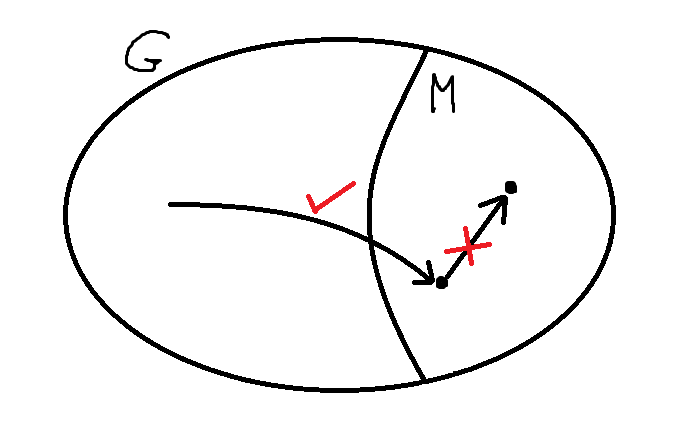
\includegraphics[width=90mm]{res/mag_abra}
	\end{center}
	
	\begin{theorem}{Mag egyértelműsége DAG-ban}{}
		Ha G véges DAG akkor G-nek pontosan egy magja van, azaz egyértelmű.
	\end{theorem}
	
	\begin{center}
		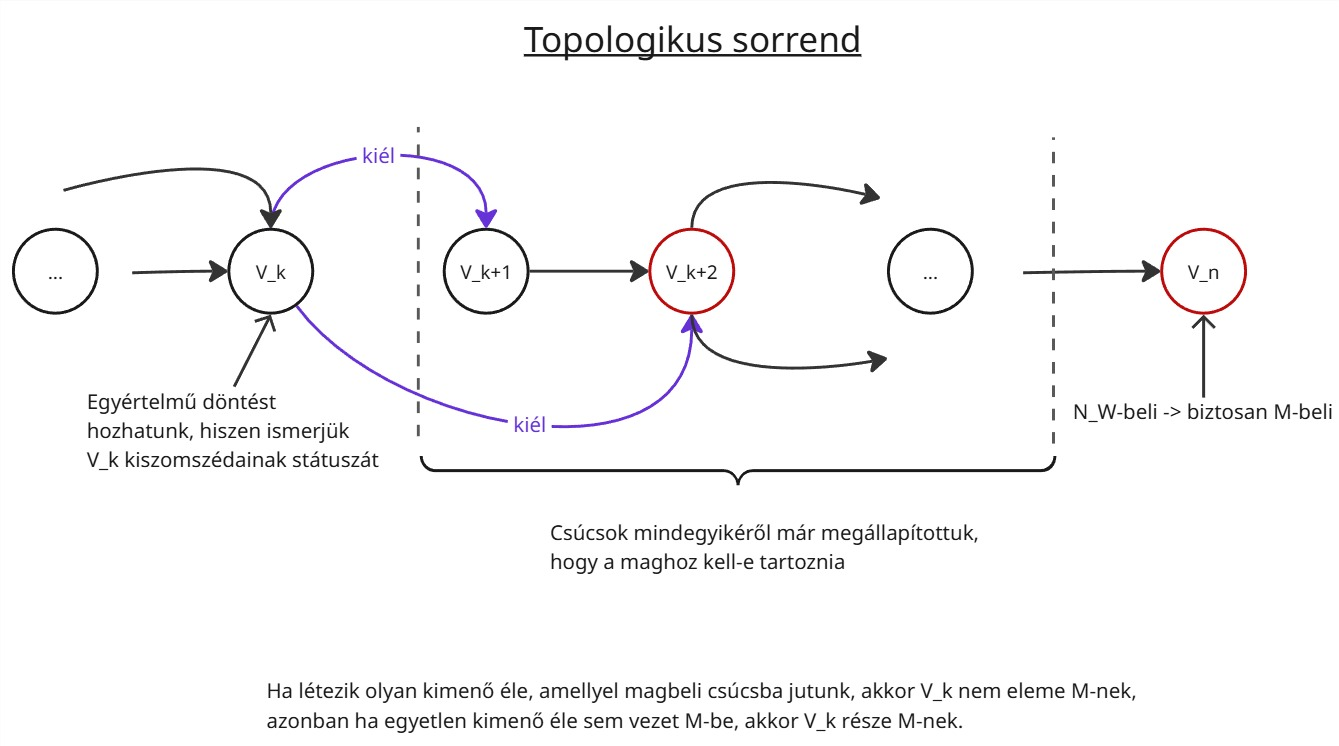
\includegraphics[width=160mm]{res/magba_tartozas.jpg}
	\end{center}
	
	\begin{definition}{Játék típusa}{}
		A $J = (v, N_W, v_0)$ éles játék típusa $v_0$.
	\end{definition}
	Ha ugyanis $v_0 \notin M$, akkor az I. játékosnak, ha pedig $v_0 \in M$, akkor viszont a II. játékosnak van nyerő stratégiája.
	
	
	\begin{definition}{Játékok összege}{}
		A $J_1 + J_2$ játék kimenetelét az utolsónak befejezett játék határozza meg.
	\end{definition}
	
	\begin{definition}{Grundy-számozás}{}
		G ir. gráfnak $g: V(G) \rightarrow \mathbb{N}$ Grundy-számozása, ha $g(v)=mex \{g(n): vu\in E(G)\}$ 
	\end{definition}
	
	\begin{observation}{}{}
		\begin{itemize}
			\item $J + J\rightarrow$ II-es típusú (másolás)
			\item $II_1 + II_2\rightarrow$ II-es típusú (mindkettőt meg tudja nyerni a 2. játékos)
			\item $I + II\rightarrow$ I-es típusú (a kezdő az I-es játékban a nyerő stratégiája szerint lép)
			\item $I + I\rightarrow$ nem egyértelmű...
		\end{itemize}
	\end{observation}
	
	\begin{statement}{}{}
		$G$ véges DAG $\Rightarrow G$-nek $\exists$! Grundy-számozása.
	\end{statement}
	Biz: $\exists$ topológikus sorrend, ebben visszafelé haladva egyértelműen adódik minden csúcsé.
	
	\begin{statement}{}{}
		Tfh. $J_1$ kezdőállapotának Grundy-száma $g_1, J_2$ kezdőállapotáé $g_2$. \\
		$J_1 + J_2$ típusa I-es, ha $g_1 \not= g_2$, és II-es ha $g_1 = g_2$.
	\end{statement}
	Biz: 
	\begin{itemize}
		\item Tfh. $g_1=g_2$. \\
		Ekkor a 2. játékos nyerni tud azzal, hogy mindig úgy lép, hogy a két állapot Grundy-száma megegyezzen.
		\item Tfh. $g_1 \not= g_2$.  \\
		Ekkor a kezdő nyer azzal, hogy a nagyobbik g-t a kisebbikre csökkenti.
	\end{itemize}
	
	
	\begin{theorem}{}{}
		$g(v_1,v_2) = g_1(v_1)\oplus g_2(v_2)$
	\end{theorem}
	
	\begin{definition}{NIM-összeadás (bitenkénti XOR)}{}
		$a \oplus b = c$ a NIM-összeadás, ahol $c$-t úgy kapjuk, hogy $a$ és $b$ 2-es számrendszerbeli alakját írásban összeadjuk, de a maradékot elfelejtjük. 
	\end{definition}
	
	\begin{observation}{NIM-összeadás tulajdonságai}{}
		\begin{itemize}
			\item $a\oplus b = b\oplus a$
			\item $(a \oplus b ) \oplus c = a \oplus (b \oplus c)$
			\item $a \oplus a = 0$
			\item $a \oplus b = a \oplus b'\Rightarrow b=b'$
			\item $c < a \oplus b \Rightarrow \exists a' < a: c =a' \oplus b$ vagy $\exists b' < b: c =a \oplus b'$
		\end{itemize}
	\end{observation}
	Biz: \\
	
	\newpage 
	\section{Előadás}
	Sprague-Grundy-tétel, Bouton tétele a NIM nyerő stratégiájáról. Játékok izomorfiája és ekvivalenciája (VKP 1.3.1). Stratégialopás (VKP 1.2), hex (VKP 1.55, 1.56).
	\begin{theorem}{Sprague–Grundy}{}
		Ha u és v $J_1 és J_2$ kombinatorikus játékokban állások, akkor $g_{J_1,J_2}(u, v) = g_{J_1}(u) \oplus g_{J_2}(v)$
	\end{theorem}
	\begin{center}
		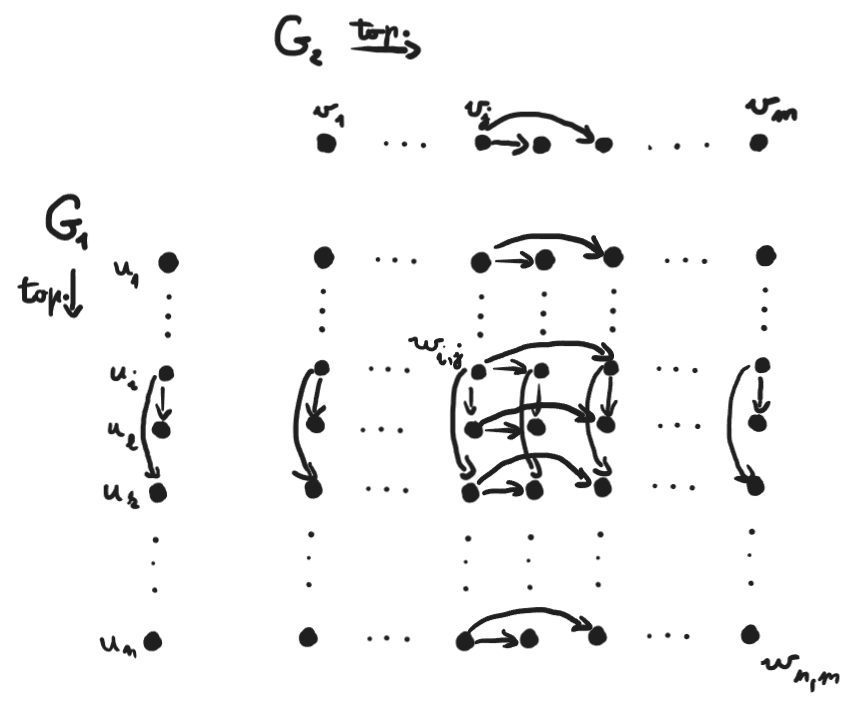
\includegraphics[width=120mm]{res/sprague-grundy_biz}
	\end{center}
	Biz.: * \\
	Teljes indukcióval:
	\begin{enumerate}
		\item $ g(w_{n,m})=g(u_n) \oplus g(v_m)$, mivel mindkettő nyelő $\Rightarrow0 = 0 \oplus 0$
		\item Tfh.: $w_{i,j}$-től jobbra és lefelé $\forall$ csúcsra teljesül (topologikus sorrend szerint)
		\item Kell: $g(w_{i,j}) = g(u_i) \oplus g(v_j)$
		\begin{enumerate}
			\item[a)] $w_{i,j} \forall z < g(u_i) \oplus g(v_j)$ értéket lát
			\item[b)] $w_{i,j}$ nem lát $ g(u_i) \oplus g(v_j)$ értéket
		\end{enumerate}
		\item[a)] Tf. indirekten, hogy $\exists z < g(u_i) \oplus g(v_j)$, hogy $w_{i,j}$ nem látja. \newline
		2.$\Rightarrow \exists g(u_i)'<g(u_i):$ $ z< g(u_i)' \oplus g(v_j)$ \newline
		$\Rightarrow u_i$ csúcsra $g(u_i)$, tehát ő látja a $g(u_i)'<g(u_i)$ értéket valamilyen $u_k$ csúcsban. \newline
		Az $u_i \rightarrow u_k$ él miatt van $w_{i,j} \rightarrow w_{k,j}$ él, és a $w_{k,j}$-re már igaz az indukciós feltétel, tehát neki $g(w_{k,j}) = g(u_i)' \oplus g(v_j) = z $, ez ellentmondás %villám jel?
		\item[b)] Tf indirekten, hogy $w_{i,j}$ lát valamilyen $w_{l,j}$-t az oszlopában.\newline
		 Az indukciós feltétel miatt $g(w_{l,j})=g(u_l) \oplus g(v_j) = g(u_i) \oplus g(v_j)$\newline
		 $\Rightarrow$ 1.$ g(u_i) = g(u_l)$, ez ellentmondás, a $g(u_i)$ nem láthat magával egyező Grundy-értéket($g(u_l))$ %villám jel?
	\end{enumerate}
	
	\begin{theorem}{Bouton}{}
		k-nim II-es típusú $\Leftrightarrow n_1 \oplus n_2 \oplus ... \oplus n_k = 0$, ahol $nn_1, ... n_k$ a kupacok méretei.
	\end{theorem}
	
	\begin{definition}{Játékok izomorfia}{}
		$J = (G, N_W, N_T, N_L, v_0)$ kombinatorikus játék izomorf $J' = (G', N_W', N_T', N_L', v_0')$ kombinatorikus játékkal, ha van olyan $G \cong G'$ gráfizomorfia, hogy $N_W$ és $N_W'$, $N_T$ és $N_T'$, $N_L$ és $N_L'$, $v_0$ és $v_0'$ egymásnak felelnek meg.
	\end{definition}
	
	\begin{definition}{Ekvivalencia}{}
		$J_1$ és $J_2$ kombinatorikus játék $u_0$ és $v_0$ kezdőpozíciókkal ekvivalensek, ha $J_1 + J_2 = II$
		
	\end{definition}
	A definícióval ekvivalens tételek:  
	\begin{itemize}
		\item $g_{J_1}(u_0) = g_{J_2}(v_0)$
		\item $\forall H$ kombinatorikus játékban igaz $H + J_1$ és $H + J_2$ azonos típusúak
	\end{itemize}

	\begin{definition}{Stratégia lopás}{}
		Bizonyítási módszer arra, hogy...
		\begin{itemize}
			\item ha nincs döntetlen, akkor az első játékosnak van nyerő stratégiája
			\item ha van döntetlen, akkor az elsőnek van nem vesztő
		\end{itemize}
	\end{definition}
	
	\begin{theorem}{Mérgezett csoki / Chomp}{}
		A kezdőjátékosnak van nyerő stratégiája
	\end{theorem}
	
	Biz.: nincs döntetlen\\
	Tegyük fel indirekt: a második játékosnak van nyerő stratégiája. Ekkor van jó válasza arra, ha a kezdő a jobb felső (n, m) kockát eszi meg. Legyen az (i, j). Lépjük ezt az (i, j) kockát első játékosként. Ezután játssza az első játékos az eredeti második nyerő stratégiája szerint.
	
	\begin{theorem}{Hex}{}
		Az első játékosnak van nyerő stratégiája
	\end{theorem}
	
	Biz.: nincs döntetlen + stratégialopás \\
	Vegyük a különböző színű mezők közötti mezőhatárokat. Írjunk ezekbe irányított éleket. \\
	Bal felső nagy nyílból kiindulva lépek az élek mentén, elakadni nem fogok, önmagába visszafordulni se, mert nem létezhet 3 irányított éllel szomszédos pont, tehát valamelyik nagy nyílba fogok elérkezni. Ekkor a kapott útnak egyik oldalon csupa azonos színű, a megfigyelt 2 térfélt összekötő utat kapunk.\\
	\begin{center}
		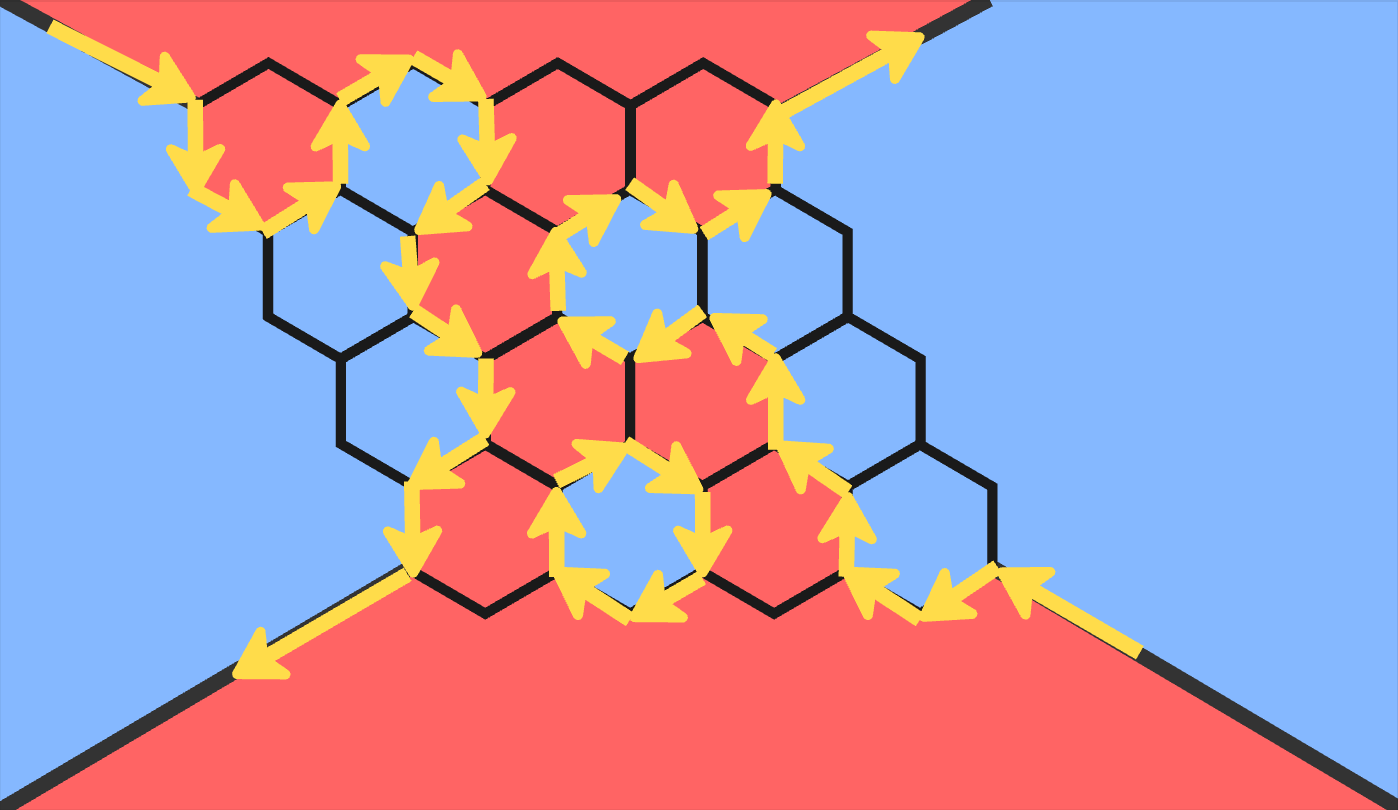
\includegraphics[width=120mm]{res/hex_biz}
	\end{center}
	
	
	\begin{theorem}{Véges amőba}{}
		Az elsőnek van nem vesztő stratégiája
	\end{theorem}
	Biz.: indirekten tegyük fel, hogy a második játékosnak van nem vesztő stratégiája \\
	Első játékos: O, második játékos: X\\
	Játsszon az első játékos egy olyan táblán, amire ő gondolatban valamilyen (i, j) mezőre egy X-et odaképzelt. Játssza ezen a képzeletbeli táblán az első játékos a második játékos nyerő stratégiáját. Ha a második pont erre az (i, j) mezőre tesz, akkor válasszon az első egy tetszőleges másik üres mezőt és képzelje oda az X-et $\rightarrowtail$ (i', j'). \\
	A játék végén: a képzelt táblán az első nem fog veszíteni, tehát a valódin sem.
	
	\newpage
	\section{Előadás}
	Stratégiai játékok, játékosok racionalitása, Pareto-optimális stratégiaválasztás. Domináns stratégiák, stratégiák (iterált) eliminálása. Tiszta Nash-egyensúly. (VKP 2, 2.1, 2.2, 2.3)
	\begin{definition}{Stratégiai játékok}{}
		$n$ játékos van, $1\leq i \leq n$ esetén $S_i$ az $i$-edik játékos lehetséges stratégiája $S = S_1 \times S_2 \times ...  \times S_n$ stratégiaválasztások (kimenetelek) halmaza.\\
		$u_i : S \longrightarrow \mathbb{R}$ i-edik játékos nyereség függvénye.
	\end{definition}
	
	\begin{remark}{Kicsit máshogy}{}
		Adott $n \in \mathbb{N}+$ játékos, és tetszőleges $i \in {1, . . . , n}$ esetén adott az $i$-edik játékoshoz
		a lehetséges stratégiáinak egy Si halmaza, valamint egy $u_i : S = S_1 \times S_2 \times ...  \times S_n \rightarrow R$ nyereségfüggvény. Minden játékos ismeri a többiek lehetséges stratégiáit és nyereségfüggvényeit. A játék egy körből
		áll, amiben a játékosok egymástól függetlenül választanak egy-egy stratégiát azzal a céllal, hogy
		maximalizálják a saját nyereségüket.
	\end{remark}
	
	$\forall$ stratégiai játékra teljesül
	\begin{itemize}
		\item 1 lépéses, szinkron ($\forall$ játékos lépése független)
		\item teljes információs ($\forall$ játékos tisztában van  $\forall$ másik játékos stratégiájával)
		\item $\forall$ játékos racionális ($\forall$ játékos a nyereségét akarja maximalizálni)
	\end{itemize}
	
	További lehetséges tulajdonságok
	\begin{itemize}
		\item 0-összegű, ha $\sum_{i=1}^{n}{}u_i(s) = 0$,  $\forall \quad s \in S$ ($u_i(s)$ az $s$ stratégiai választás nyersége/költsége)
		\item szimmetrikus, ha $\exists k$, amire $|S_i|= k$ és ezek a stratégiák megszámlálhatók úgy 1-től k-ig, hogy $\forall \pi$ permutációra [n]-en $\forall \quad 1\leq i \leq n \quad v_i(s)=u_{\pi (i)}(s_{\pi}) \quad \forall s \in S$
	\end{itemize}
	
	\begin{definition}{Kő-Papír-Olló}{}
		\begin{itemize}
			\item 0 összegű (minden cella összege 0)
			\item szimmetrikus
		\end{itemize}
	\end{definition}
	
	\begin{center}
		\begin{tabular}{llll}
			\hline
			\multicolumn{1}{|l|}{}  & \multicolumn{1}{l|}{K}     & \multicolumn{1}{l|}{P}     & \multicolumn{1}{l|}{O}     \\ \hline
			\multicolumn{1}{|l|}{K} & \multicolumn{1}{l|}{0, 0}  & \multicolumn{1}{l|}{-1, 1} & \multicolumn{1}{l|}{1, -1} \\ \hline
			\multicolumn{1}{|l|}{P} & \multicolumn{1}{l|}{1, -1} & \multicolumn{1}{l|}{0, 0}  & \multicolumn{1}{l|}{-1, 1} \\ \hline
			\multicolumn{1}{|l|}{O} & \multicolumn{1}{l|}{-1, 1} & \multicolumn{1}{l|}{1, -1} & \multicolumn{1}{l|}{0, 0}  \\ \hline
			\multicolumn{4}{l}{Kő-papír-olló strat. mátrix}                                                               
		\end{tabular}
	\end{center}
	
	
	
	\begin{definition}{Fogolydilemma}{}
		\begin{itemize}
			\item $\varepsilon > 0 $ kis szám
			\item nem 0 összegű
			\item szimmetrikus
			\item az önzés a racionális döntés
		\end{itemize}
	\end{definition}
	
	\begin{center}
		\begin{tabular}{lll}
			\hline
			\multicolumn{1}{|l|}{}     & \multicolumn{1}{l|}{önző}              & \multicolumn{1}{l|}{koop}         \\ \hline
			\multicolumn{1}{|l|}{önző} & \multicolumn{1}{l|}{-100 + $\varepsilon$, -100 +$\varepsilon$} & \multicolumn{1}{l|}{-1 + $\varepsilon$, -100} \\ \hline
			\multicolumn{1}{|l|}{koop}    & \multicolumn{1}{l|}{-100, -1 + $\varepsilon$}      & \multicolumn{1}{l|}{-1, -1}       \\ \hline
			\multicolumn{3}{l}{Fogoly-dilemma}                                                                     
		\end{tabular}
	\end{center}
	
	\begin{definition}{Dominálás}{}
		$ 1 \leq i \leq n \quad  s,s' \in S_i$, $s$ dominálja $s'$-t, ha $ \forall\quad z \in S_{-i} : u_i(s,z) > u_i(s',z)$,
		 ahol $S_{-i} = S_1\times ... \times S_{i-1} \times S_{i+1} \times ... \times S_{n}$.
		 \begin{itemize}
		 	\item Ez gyenge dominálás, ha $  u_i(s,z) \geq u_i(s',z)$
		 	\item $s$ az i. játékosé, $z$ mindenki más stratégiája
		 \end{itemize}
	\end{definition}
	
	\begin{definition}{Gyenge dominálás}{}
		Az $i.$ játékos $z \in S_i$ stratégiája gyengén dominálja a $z' \in S_i$ stratégiáját, ha a többi játékos tetszőleges $s_1 \in S_1, ..., s_{i-1} \in S_{i-1}, s_{i+1} \in S_{i+1}, ..., s_n \in S_n$ stratégiaválasztás esetén  
		\begin{center}
			$u_i(s_1, ..., s_{i-1}, z, s_{i+1}, ..., s_n) \geq u_i(s_1, ..., s_{i-1}, z', s_{i+1}, ..., s_n)$.
		\end{center}
	\end{definition}
	
	\begin{definition}{Erős dominálás}{}
		Az $i.$ játékos $z \in S_i$ stratégiája gyengén dominálja a $z' \in S_i$ stratégiáját, ha a többi játékos tetszőleges $s_1 \in S_1, ..., s_{i-1} \in S_{i-1}, s_{i+1} \in S_{i+1}, ..., s_n \in S_n$ stratégiaválasztás esetén  
		\begin{center}
			$u_i(s_1, ..., s_{i-1}, z, s_{i+1}, ..., s_n) > u_i(s_1, ..., s_{i-1}, z', s_{i+1}, ..., s_n)$.
		\end{center}
	\end{definition}
	
	\begin{definition}{Százlábú játék}{}
		\begin{itemize}
			\item 2 játékos
			\item lépéskor: kiszáll/játszik tovább
			\item $(n,m)$: $n$ az első játékos, $m$ a második játékos nyeresége 
			\item minden lépésnél a racionális döntés kiszállni
		\end{itemize}
	\end{definition}
	\begin{center}
		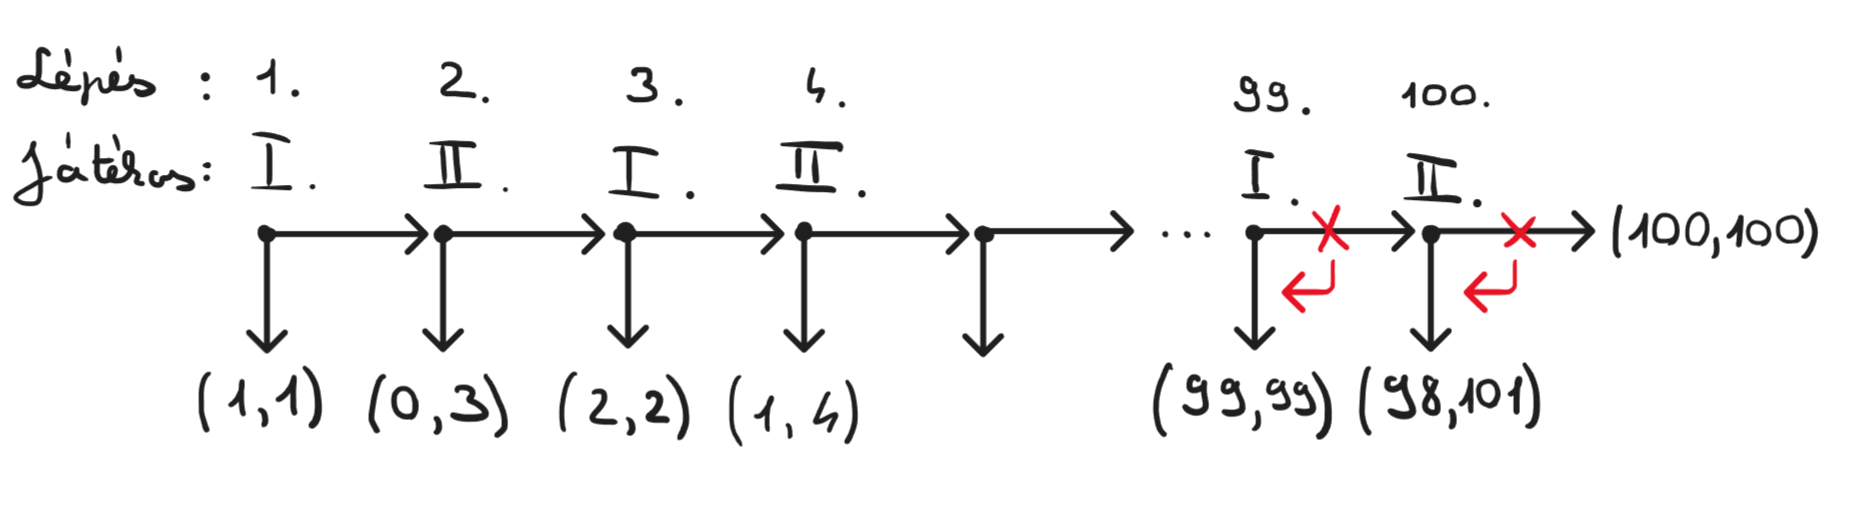
\includegraphics[width=160mm]{res/szazlabu_abra}
	\end{center}
	
	\begin{definition}{Iterált szigorú eliminálás}{}
		A játékban részt vevő bármely játékos erősen dominált stratégiáját töröljük, és ezt ismételjük mindaddig, amíg van olyan játékos, akinek maradt még erősen dominált
		stratégiája.
	\end{definition}
	
	\begin{definition}{Iterált laza eliminálás}{}
		A játékban részt vevő bármely játékos gyengén dominált stratégiáját töröljük, és ezt ismételjük mindaddig, amíg van olyan játékos, akinek maradt még gyengén dominált
		stratégiája.
	\end{definition}
	
	\begin{theorem}{}{}
		Iterált szigorú eliminálásokat végezve, amíg lehet, mindig ugyanazt a játékot kapjuk.
	\end{theorem}
	Biz.:\\
	Tfh.: $s_1, s_2, ... s_l$ sorrendben szigorúan eliminálva további elimináció nem végezhető, ill. $z_1, z_2, ... z_t$ stratégiákra ugyanezt. Cél $\{ s_1, s_2, ... s_l\} = \{z_1, ... z_t\}$\\
	Indirekt: Tfh. $\neq$, azaz  $\exists s_i \notin \{z_1, ... z_t\}$\\
	Legyen $i$ min erre!\\
	$s_1, s_2, ... s_{i-1} \in \{z_1, z_2 ... z_t\} \Longrightarrow z$ eliminálása után $s_i$ dominált.
	
	\begin{definition}{Pareto dominálás}{}
		$s, s' \in S, \quad s \quad$Pareto-dominálja s'-t, ha $u_i(s) \geq u_i(s') \quad \forall i \in [n]$ és $\exists j \in [n] : u_j(s) > u_j(s')$.
	\end{definition}
	pl. Fogoly dilemmában
	
	\begin{definition}{Pareto-optimális stratégiaválasztás}{}
		$s \in S$ strat. választás Pareto-optimális, ha semelyik más strat. választás sem Pareto-dominálja.
	\end{definition}
	
	\begin{remark}{Kicsit másképp}{}
		Az $(s_1, ..., s_n) \in S_1 \times ... \times S_n$ stratégiaválasztás Pareto-optimális, ha nem létezik olyan $(s'_1, ..., s'_n) \in S_1 \times ... \times S_n$ stratégiaválasztás, melyre a következők teljesülnek:
		\begin{itemize}
			\item minden $i \in \{1, ..., n\}$ esetén $u_i(s_1, ..., s_n) \leq u_i(s'_1, ..., s'_n)$, és
			\item létezik olyan $j \in \{1, ..., n\}$ esetén $u_j(s_1, ..., s_n) \leq u_j(s'_1, ..., s'_n)$
		\end{itemize}
	\end{remark}
	pl. Kő - Papír - Olló lépései
	
	[diagram]
	
	\begin{definition}{Nash-egyensúly (NE)}{}
		$s \in S$ tiszta Nash-egyensúly, ha egyetlen játékosnak sem érdeke más stratégiát választani azaz $u_i(s) \geq u_i(s',s_{-i}) \quad \forall \; 1 \leq i \leq n \quad \forall s' \in S_i$ \\
		Az $(s_1, ..., s_n) \in S_1 \times ... \times S_n$ stratégiaválasztás tiszta Nash-egyensúly, ha minden $i \in \{1, ..., n\}$ és $s'_i \in S_i$ esetén
		\begin{center}
			$u_i(s_1, ..., s_{i-1}, s_i, s_{i+1}, ..., s_n) \geq u_i(s_1, ..., s_{s-1}, s'_i, s_{i+1}, ..., s_n)$
		\end{center}
	\end{definition}
	Példa: fogoly-dillemmában van ilyen, kő-papír-ollóban nincs
	
	\begin{theorem}{(iterált) eliminálás
			hatása a Nash-egyensúlyokra}{}
		Szig. elim. hatására a tiszta NE-k (tNE) halmaza nem változik
	\end{theorem}
	Biz.: [...] \\
	Tfh.: $s \in S_i$ dominálja $s' \in S_i$-t és $s'$-t töröljük
	
	\begin{observation}{}{}
		Törlés előtt tNE nem tartalmazta s'-t 
	\end{observation}
	Következmény: $\forall$ törlés tNE a törlés után is tNE marad \\
	Tfh.: z tNE a törlés után. Ha z nem tNE a törlés előtt $u_i(s', z_{-i}) > u_i(z)$
	
	\newpage
	\section{Előadás}
	Kevert Nash-egyensúly, maximin stratégia és Nash-egyensúly kapcsolata.(VKP 2.4, 2.6)
	\begin{definition}{Kevert stratégia}{}
		$\sigma_i : S_i \rightarrow \mathbb{R}_+$ kevert stratégia, ha $\sum_{s_i \in S_i} \sigma_i(s_i) = 1$ \\
		$\Delta_i$: ezek halmaza $\rightarrow$ i-dik játékos kevert stratégiái 
		$s_i \in S_i$-hez tartozó tiszta stratégia \\
		$\chi_{s_i}$-vel jelöljük: 
		\[
		\chi_{s_i}(s') =
		\begin{cases}
			1 & s' = s_i, \\
			0 & s' \neq s_i
		\end{cases}
		\] 
		$\Delta = \Delta_1 \times , ..., \times \Delta_n$: kevert stratégia választások halmaza \\
		$\sigma \in \Delta$ (kevert strat. választás), \quad $s \in S$ (konkrét strat. választás) ($\rightarrow$ rögzítünk egy konkrét strat. választást) $P_\sigma (s) = \prod_{i=1}^n \sigma_i(s_i) $ (független események)\\
		$\sigma = (\sigma_1, ..., \sigma_n) \quad s=(s_1, ..., s_n) \quad u_i(\sigma) = \sum_{s \in S} P_\sigma (s) \cdot u_i(s)$ i-dik  játékos nyeresége, várható nyereség
	\end{definition}
	
	\begin{definition}{Legjobb válasz}{}
		$s_{-i} = (s_1, ..., s_n) \in S_{-i},$ (i-dik játékos kivételével mindenkinek választottunk stratégiát) esetén $s_i$ az i-dik játékos számára legjobb válasza, ha $u_i(s_i,s_{-i}) \geq u_i(s_i',s_{-i}) \quad \forall s'_i \in S$
	\end{definition}
	
	Láttuk: $s \in S$ tNE, ha $\forall$ i-re $s_i$ legjobb válasza $s_i$-re, ahol $s = (s_1, ..., s_n)$
	
	\begin{definition}{Legjobb kevert válasz}{}
		$\sigma_{-i} \in \Delta_{-i}$ esetén $s_i \in S$ az i-dik játékos számára legjobb tiszta stratégiai választás, ha $u_i(s_i, \sigma_{-i}) \geq u_i(s_i',\sigma_{-i}) \quad \forall s_i' \in S_i$-re
	\end{definition}
	
	$\sigma_i$ az i-dik játékos számára legjobb kevert stratégia, ha $u_i(\sigma_i, \sigma_{-i}) \geq u_i(\sigma_i', \sigma_{-i})$
	
	\begin{observation}{Legjobb tiszta válasz}{}
		$\sigma_i$ az i-dik játékos számára legjobb kevert strat. $\Leftrightarrow \quad \sigma_i = \sum_{s \in S_i} \lambda_s \chi_s$, ahol $\lambda_s > 0$ esetén s legjobb tiszta válasz
	\end{observation}
	
	Biz.: [...]
	
	\begin{definition}{Kevert Nash-egyensúly (kNE)}{}
		$\sigma = (\sigma_1, ..., \sigma_n) \in \Delta$ kevert Nash-egyensúly, ha $\sigma_i$ legjobb kevert válasz $\sigma_{-i}$-re $\forall 1\leq i \leq n$
	\end{definition}
	
	Pl.: kő-papír-olló
	\begin{center}
		\begin{tabular}{llll}
			\hline
			\multicolumn{1}{|l|}{}  & \multicolumn{1}{l|}{K}     & \multicolumn{1}{l|}{P}     & \multicolumn{1}{l|}{O}     \\ \hline
			\multicolumn{1}{|l|}{K} & \multicolumn{1}{l|}{0, 0}  & \multicolumn{1}{l|}{-1, 1} & \multicolumn{1}{l|}{1, -1} \\ \hline
			\multicolumn{1}{|l|}{P} & \multicolumn{1}{l|}{1, -1} & \multicolumn{1}{l|}{0, 0}  & \multicolumn{1}{l|}{-1, 1} \\ \hline
			\multicolumn{1}{|l|}{O} & \multicolumn{1}{l|}{-1, 1} & \multicolumn{1}{l|}{1, -1} & \multicolumn{1}{l|}{0, 0}  \\ \hline
			\multicolumn{4}{l}{Kő-papír-olló strat. mátrix}                                                               
		\end{tabular}
	\end{center}
	
	\begin{center}
		$\sigma_1 = (1/3, 1/3, 1/3) \quad \sigma_2 = (1/3, 1/3, 1/3)$
	\end{center}
	
	\[\text{legjobb tiszta válaszok}
	\begin{cases}
		u_1(k, \sigma_2) = 1/3(0+1-1)=0 \\
		u_1(k, \sigma_2) = 1/3(1+0-1)=0 \\
		u_1(k, \sigma_2) = 1/3(-1+1+0)=0
	\end{cases}
	\]
	
	\begin{theorem}{}{}
		$\forall$ strat játéknak van kevert Nash-egyensúlya
	\end{theorem}
	
	Nem bizonyítjuk
	
	\begin{definition}{}{}
		$\sigma_i \in \Delta_i$ erősen dominálja az $s \in S_i$ stratégiát, ha $u_i(\sigma_i, \sigma_{-i}) > u_i(s, \sigma_{-i}) \quad \forall \sigma_{-i} \in \Delta_{-i}$
	\end{definition}
	
	\begin{definition}{}{}
		$\sigma_i \in \Delta_i$ gyengén dominálja az $s \in S_i$ stratégiát, ha $u_i(\sigma_i, \sigma_{-i}) \geq u_i(s, \sigma_{-i}) \quad \forall \sigma_{-i} \in \Delta_{-i}$
	\end{definition}
	
	\begin{center}
		\begin{tabular}{|l|l|l|l|l|}
			\hline
			$u_2$ & $s_1$ & $s_2$ & $s_3$ & $\sigma_2$ \\ \hline
			$z_1$ & 3    & 0    & 1    & 1,5                      \\ \hline
			$z_2$ & 0    & 3    & 1    & 1,5                      \\ \hline
		\end{tabular}
	\end{center}
	
	\begin{center}
		$\sigma_2 = 1/2 \chi_{s_1} + 1/2 \chi_{s_2}$
	\end{center}
	
	\begin{definition}{Szigorú / laza eliminálás}{}
		erősen / gyengén dominált stratégia törlése
	\end{definition}
	
	\begin{definition}{}{}
		Iterált szigorú / laza eliminálás ...
	\end{definition}
	
	\begin{statement}{}{}
		Szigorú eliminálással kNE nem tűnik el
	\end{statement}
	
	Biz.: [...]
	
	\begin{statement}{}{}
		Laza eliminálás után kapott kNE az eliminálás előtti játékban is kNE
	\end{statement}
	
	Biz.: [...] \\
	
	Köv.: iterált szigorú eliminálás nem változtatja a kNE-ok halmazát. \\ 
	
	Példa: Játék: Ha a két szám megegyezik az összeget a sorjátékos nyeri meg, ha nem, az oszlopjátékos
	
	\begin{center}
		\begin{tabular}{llll}
			&                            & \multicolumn{2}{c}{II.}                                 \\ \cline{2-4} 
			\multicolumn{1}{l|}{}   & \multicolumn{1}{l|}{}      & \multicolumn{1}{l|}{a = 1} & \multicolumn{1}{l|}{b = 2} \\ \cline{2-4} 
			\multicolumn{1}{l|}{I.} & \multicolumn{1}{l|}{x = 1} & \multicolumn{1}{l|}{2, 0}  & \multicolumn{1}{l|}{0, 3}  \\ \cline{2-4} 
			\multicolumn{1}{l|}{}   & \multicolumn{1}{l|}{y = 2} & \multicolumn{1}{l|}{0, 3}  & \multicolumn{1}{l|}{4, 0}  \\ \cline{2-4} 
		\end{tabular}
	\end{center}
	
	\begin{figure}[h]
		\centering
		\begin{minipage}{0.45\textwidth}
			\centering
			% első ábra
			
			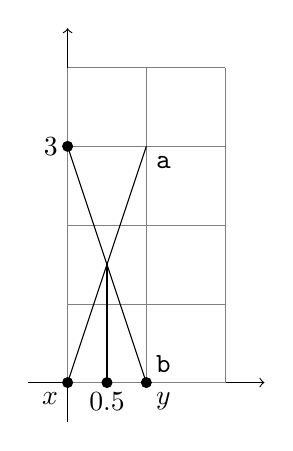
\begin{tikzpicture}[scale=1]
				% tengelyek
				\draw[->] (-0.5,0) -- (2.5,0);
				\draw[->] (0,-0.5) -- (0,4.5);
				
				% rácsvonalak (opcionális)
				\draw[step=1cm,gray,very thin] (0,0) grid (2,4);
				
				% pont és felirat
				\fill (0.5,0) circle (2pt) node[below] {$0.5$};
				\fill (0,3) circle (2pt) node[left] {$3$};
				\fill (0,0) circle (2pt) node[below left] {$x$};
				\fill (1,0) circle (2pt) node[below right] {$y$};
				\draw (1,3) node[below right] {\texttt{a}};
				\draw (1,0) node[above right] {\texttt{b}};
				
				%line
				\draw (0,0) -- (1,3);
				\draw (0,3) -- (1,0);
				\draw (0.5,0) -- (0.5,1.5);
				
			\end{tikzpicture}
			\caption{Oszlopjátékos}
		\end{minipage}
		\hfill
		\begin{minipage}{0.45\textwidth}
			\centering
			% második ábra
			
			\begin{tikzpicture}[scale=1.5]
				% tengelyek
				\draw[->] (-0.5,0) -- (2.5,0);
				\draw[->] (0,-0.5) -- (0,2.5);
				
				% rácsvonalak (opcionális)
				\draw[step=1cm,gray,very thin] (0,0) grid (2,2);
				
				% pont és felirat
				\fill (0.5,0)  node[below] {$0.5$};
				\fill (0,0) node[below left] {$x$};
				\fill (1,0) node[below right] {$y$};
				
				%line
				\draw[very thick] (0,1) -- (0.5,1);
				\draw[very thick] (0.5,1) -- (0.5,0);
				\draw[very thick] (0.5,0) -- (1,0);
				
			\end{tikzpicture}
		\end{minipage}
	\end{figure}
	
	\begin{figure}[h]
		\centering
		\begin{minipage}{0.45\textwidth}
			\centering
			% első ábra
			
			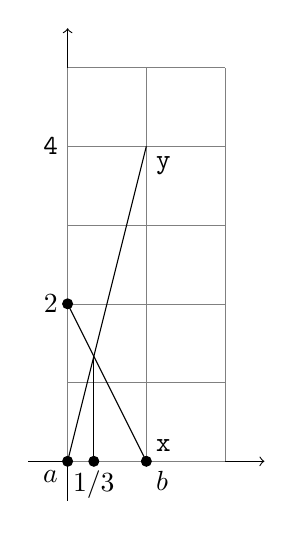
\begin{tikzpicture}[scale=1]
				% tengelyek
				\draw[->] (-0.5,0) -- (2.5,0);
				\draw[->] (0,-0.5) -- (0,5.5);
				
				% rácsvonalak (opcionális)
				\draw[step=1cm,gray,very thin] (0,0) grid (2,5);
				
				% pont és felirat
				\fill (0,0) circle (2pt) node[below left] {$a$};
				\fill (1,0) circle (2pt) node[below right] {$b$};
				\fill (0.333,0) circle (2pt) node[below] {$1/3$};
				\fill (0,2) circle (2pt) node[left] {$2$};
				
				\draw (0,4) node[left] {\texttt{4}};
				\draw (1,4) node[below right] {\texttt{y}};
				\draw (1,0) node[above right] {\texttt{x}};
				
				%line
				\draw (0,0) -- (1,4);
				\draw (0,2) -- (1,0);
				\draw (0.333,0) -- (0.333,1.333);
				
			\end{tikzpicture}
			\caption{Sorjátékos}
		\end{minipage}
		\hfill
		\begin{minipage}{0.45\textwidth}
			\centering
			% második ábra
			
			\begin{tikzpicture}[scale=1.5]
				% tengelyek
				\draw[->] (-0.5,0) -- (2.5,0);
				\draw[->] (0,-0.5) -- (0,2.5);
				
				% rácsvonalak (opcionális)
				\draw[step=1cm,gray,very thin] (0,0) grid (2,2);
				
				% pont és felirat
				\fill (0,0) node[below left] {$a(0)$};
				\fill (1,0) node[below right] {$b(1)$};
				\fill (0.333,0) node[below] {$1/3$};
				
				
				%line
				\draw[very thick] (0,0) -- (0.333,0);
				\draw[very thick] (0.333,0) -- (0.333,1);
				\draw[very thick] (0.333,1) -- (1,1);
				
			\end{tikzpicture}
		\end{minipage}
	\end{figure}
	
	\begin{figure}[h]
		\centering
		\begin{minipage}{0.45\textwidth}
			\centering
			\begin{tikzpicture}[scale=3]
				% tengelyek
				\draw[->] (-0.5,0) -- (1.5,0);
				\draw[->] (0,-0.5) -- (0,1.5);
				
				% rácsvonalak (opcionális)
				\draw[step=1cm,gray,very thin] (0,0) grid (1,1);
				
				% pont és felirat
				\fill (0,0) node[below left] {$a$};
				\fill (1,0) node[below right] {$b$};
				
				\fill (0,0) node[above left] {$x$};
				\fill (0,1) node[above left] {$y$};
				
				\fill (0.333,0) node[below] {$1/3$};
				\fill (0,0.5) node[left] {$1/2$};
				
				%line
				\draw[very thick] (0,0) -- (0.333,0);
				\draw[very thick] (0.333,0) -- (0.333,1);
				\draw[very thick] (0.333,1) -- (1,1);
				
				\draw[very thick] (0,1) -- (0,0.5);
				\draw[very thick] (0,0.5) -- (1,0.5);
				\draw[very thick] (1,0.5) -- (1,0);
				
				%
				\draw (0.333,0.5) circle (2pt);
				
			\end{tikzpicture}
		\end{minipage}%
		\hfill
		\begin{minipage}{0.45\textwidth}
			$\sigma_1 = 1/3 \chi_b + 2/3\chi_a$ \\
			$\sigma_2=1/2\chi_x+1/2\chi_y$
		\end{minipage}
	\end{figure}
	
	\newpage
	\newpage
	\section{Előadás}
	0-összegű kétszemélyes játékok kevert Nash-egyensúlya lineáris programozási feladatként, Neumann-tétel. (VKP 2.7)
	Csődjáték, kelmeszabály-konzisztens szétosztás, Kaminski-féle közlekedőedény-rendszer, a csődjáték nukleolusza (T 9.3, (VKP 4.1))
	\begin{definition}{Maximin stratégia}{}
		Strat. játék esetén az i-dik játékos maximin stratégiája egy olyan $\sigma_1 \in \Delta$ kevert stratégiája, amire $min u_i(\sigma_i, s_{-i}) \geq min u_i (\sigma_i, \sigma_{-i}) \quad \forall \sigma_i \in \Delta_i$
	\end{definition}
	
	\begin{center}
		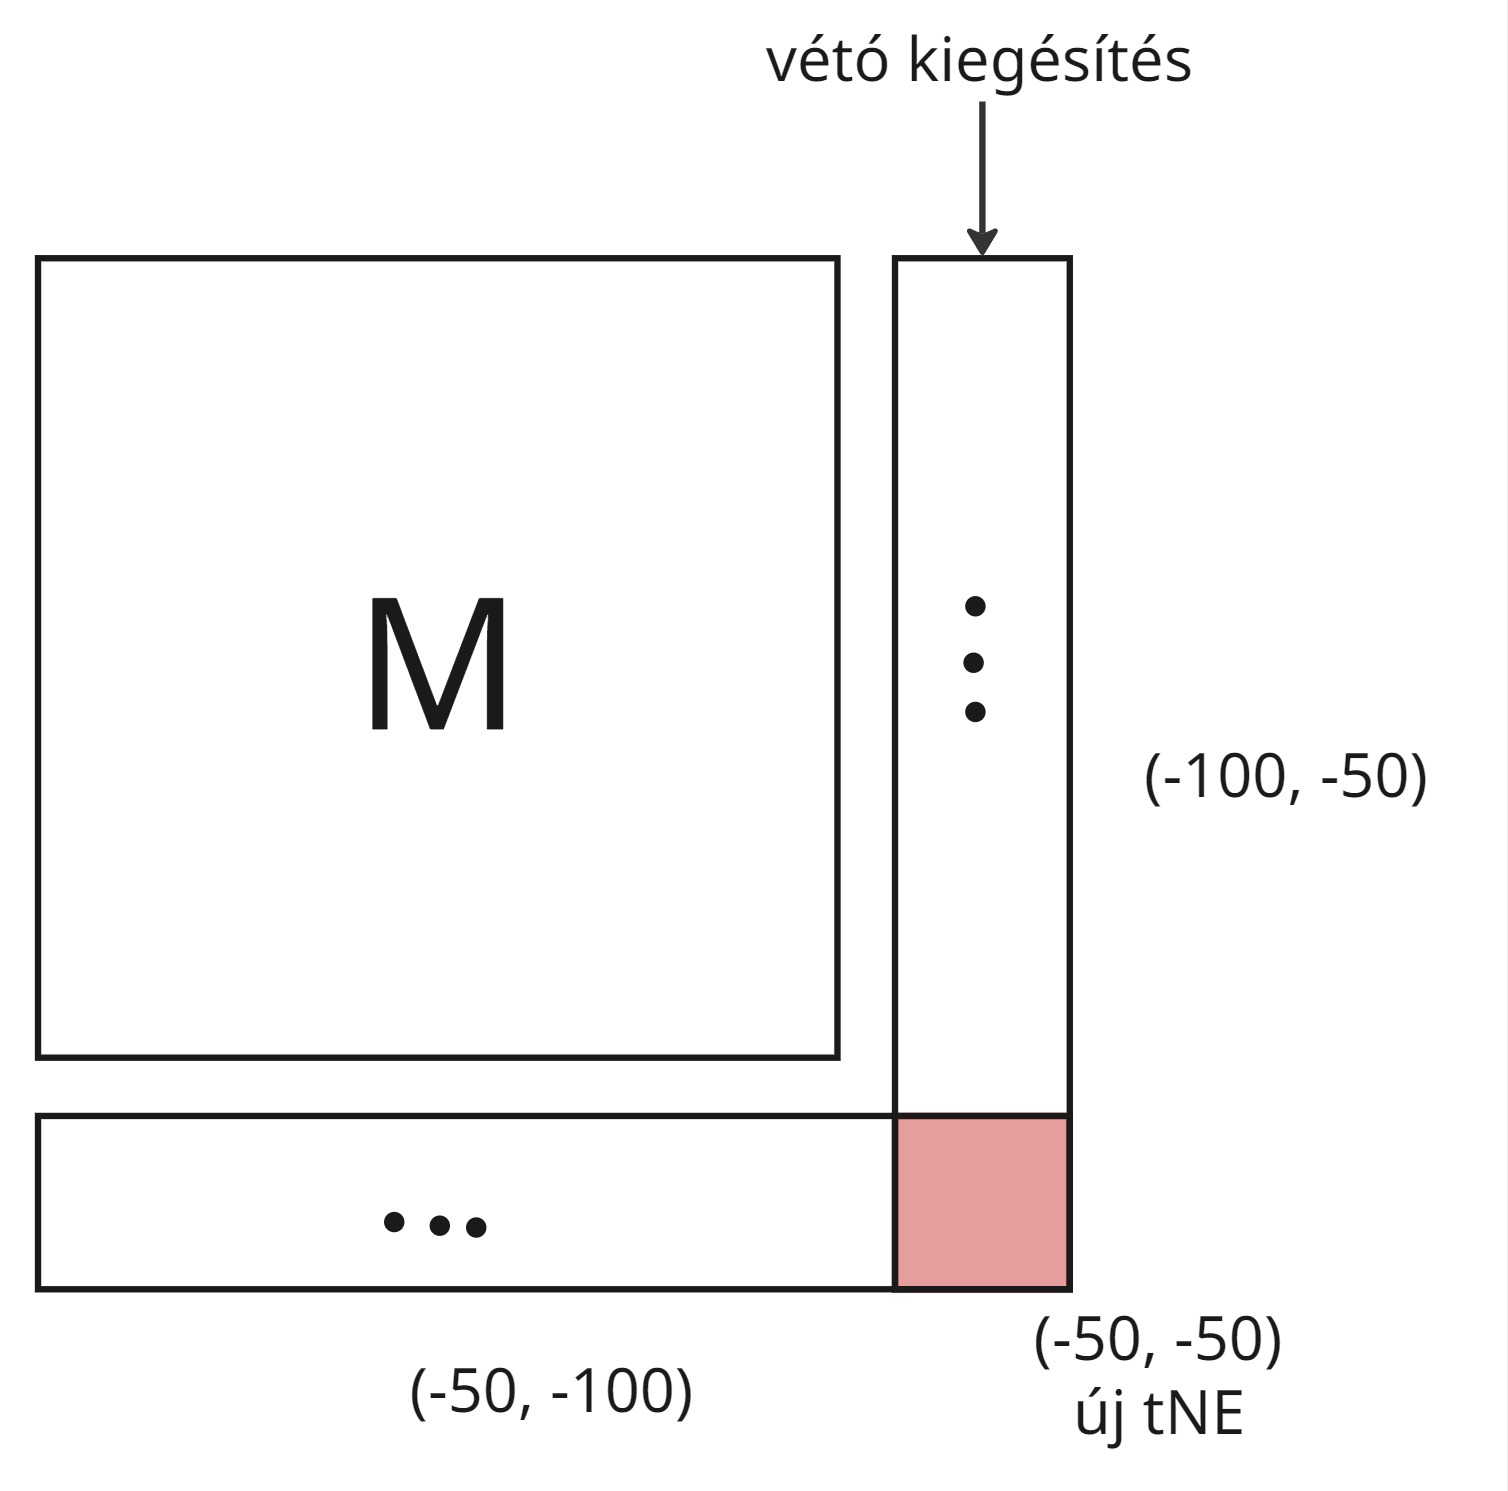
\includegraphics[width=90mm]{res/veto_kieg.jpg}
	\end{center}
	
	\begin{observation}{}{}
		\begin{enumerate}
			\item A maximin stratégiaválasztása általában nem kNE
			\item Mindig van maximin stratégia, és ez egy Lineáris Programozási feladat megoldásával kapható
		\end{enumerate}
	\end{observation}
	
	
	
	\begin{definition}{Standard LP feladat}{}
		$max c(x), ahol A \times x \leq b$
	\end{definition}
	
	\begin{center}
		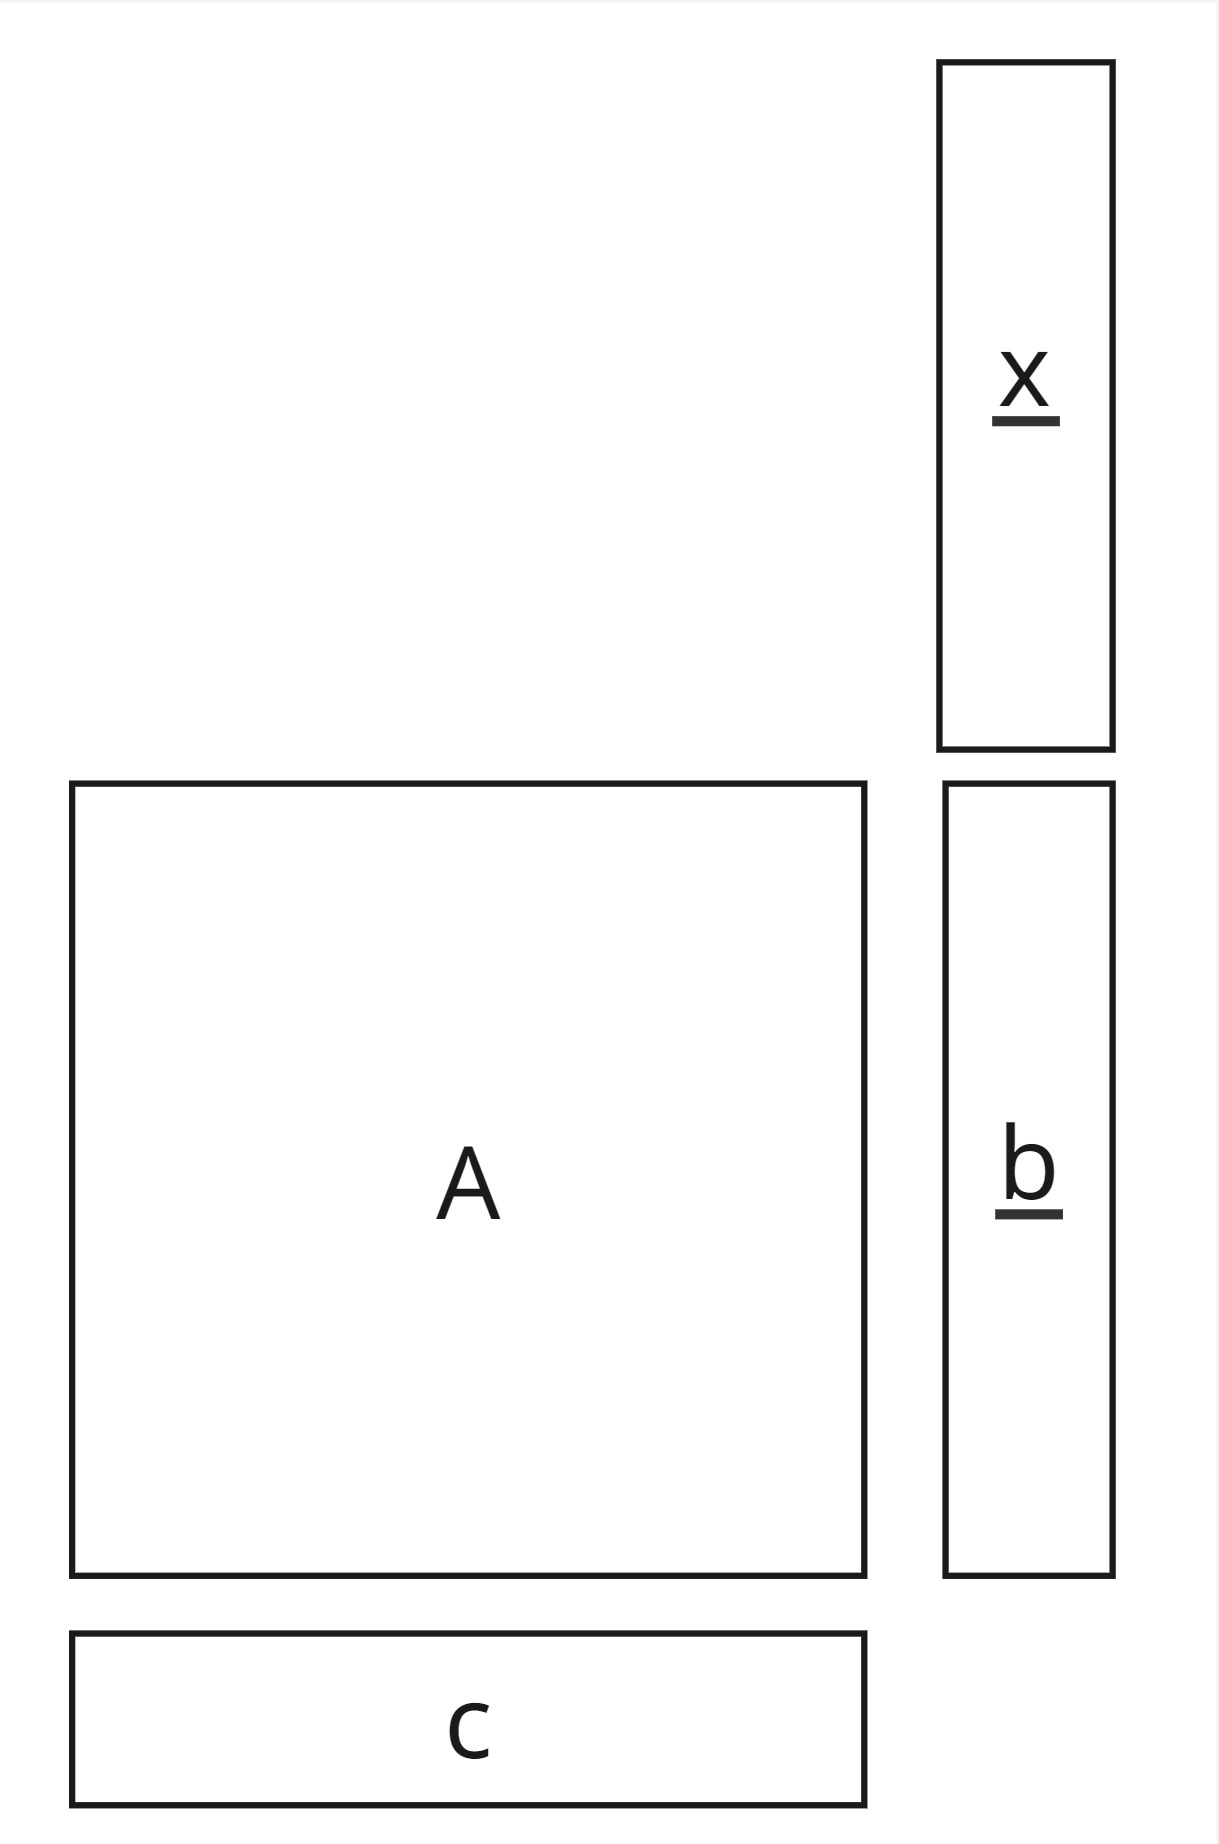
\includegraphics[width=50mm]{res/standardLP.jpg}
	\end{center}
	
	\begin{definition}{Oszlopjátékos maximin stratégiájának keresése}{}
		Milyen valószínűséggel választunk egy oszlop kevert stratégiát 
		\[\text{Biztonsági szint : max}
		\begin{cases}
			\alpha : M \cdot x \geq \alpha \cdot 1\\
			1^T \cdot x = 1, x \geq 0
		\end{cases}
		\]
	\end{definition}
	[javítás alatt]
	%\begin{center}
	%	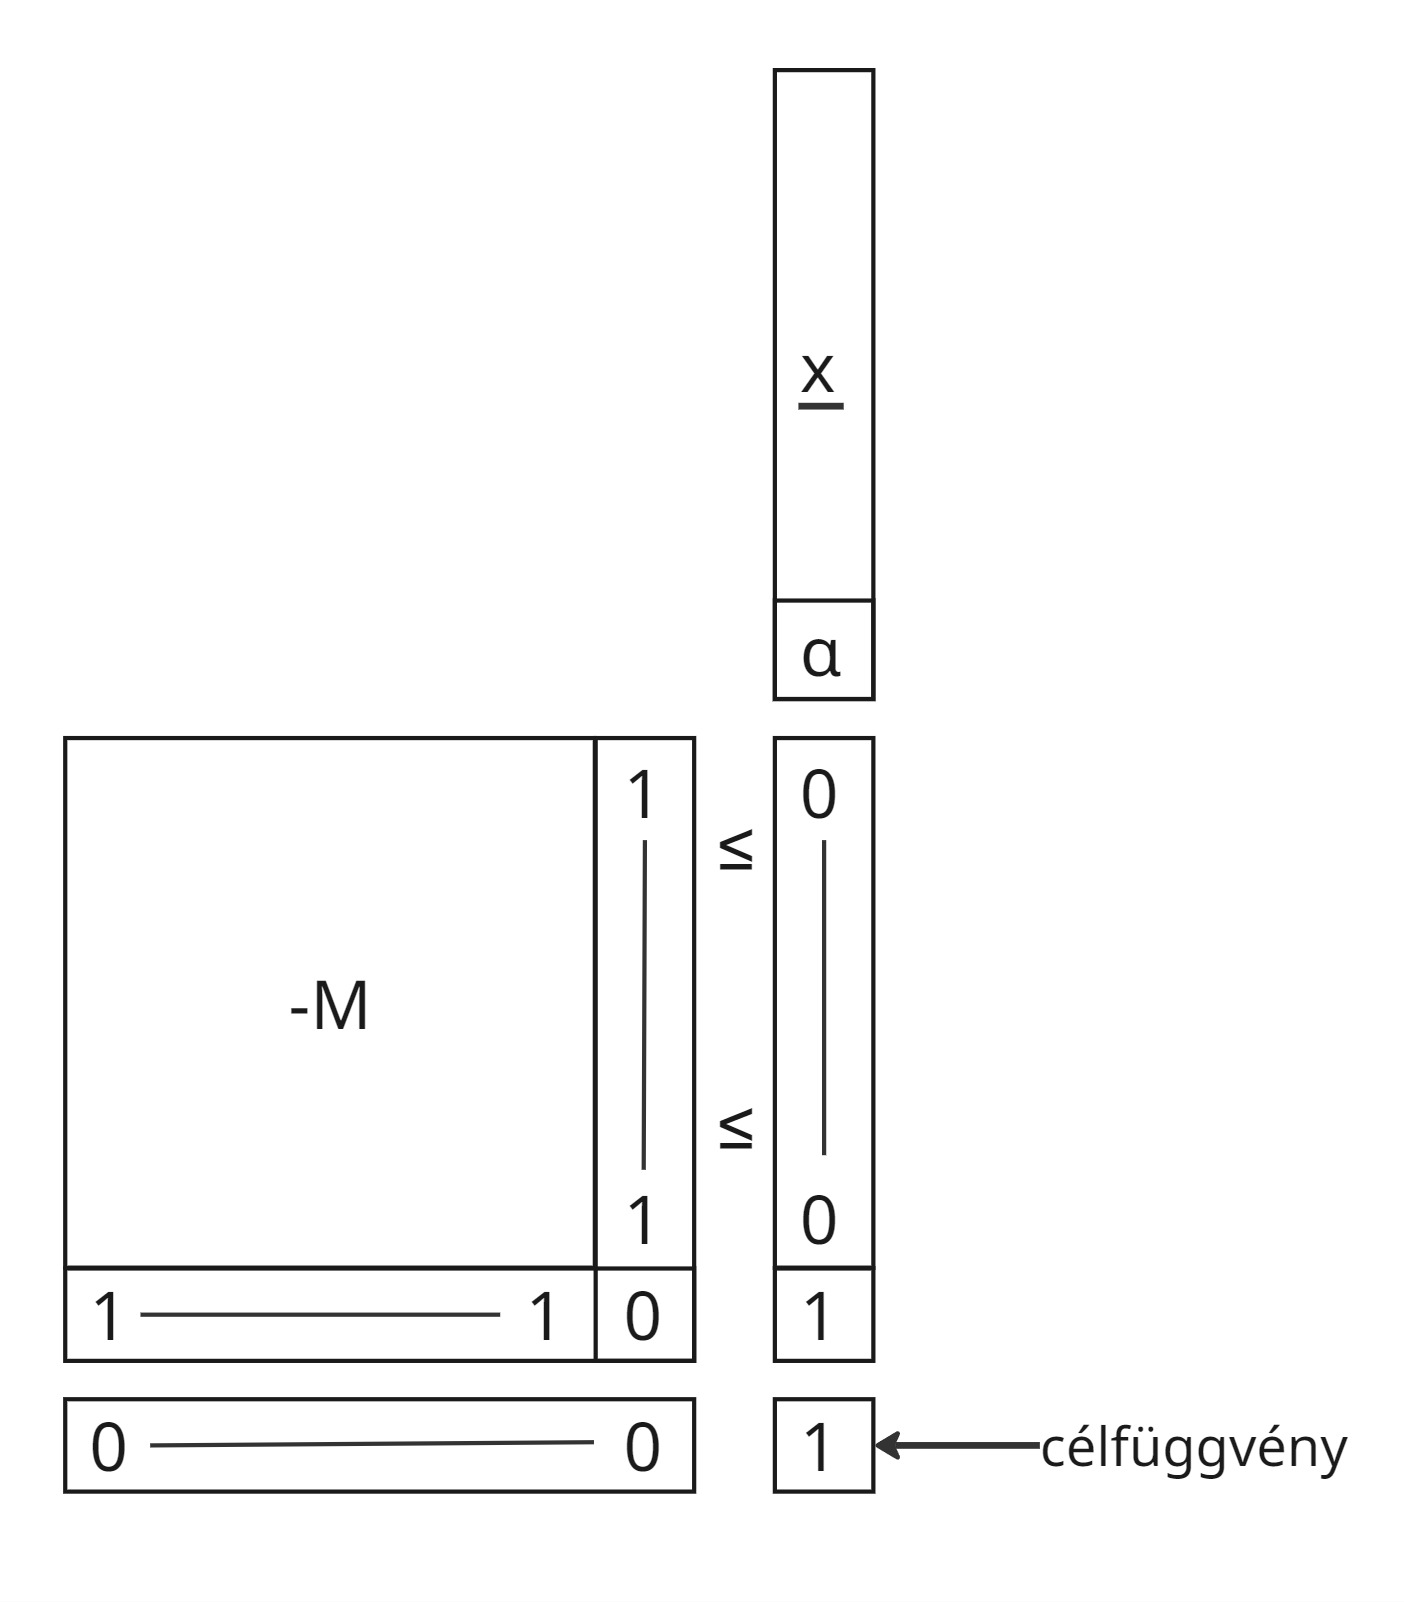
\includegraphics[width=90mm]{res/oszlop_maximin.jpg}
	%\end{center}
	
	\begin{theorem}{Neumann-tétel}{}
		2 személyes 0-összegű játék esetén a sorjátékos biztonsági szintje megegyezik az oszlopjátékos biztonsági szintjének (-1)-szeresével
	\end{theorem}
	[javítás alatt]
	%\begin{center}
	%	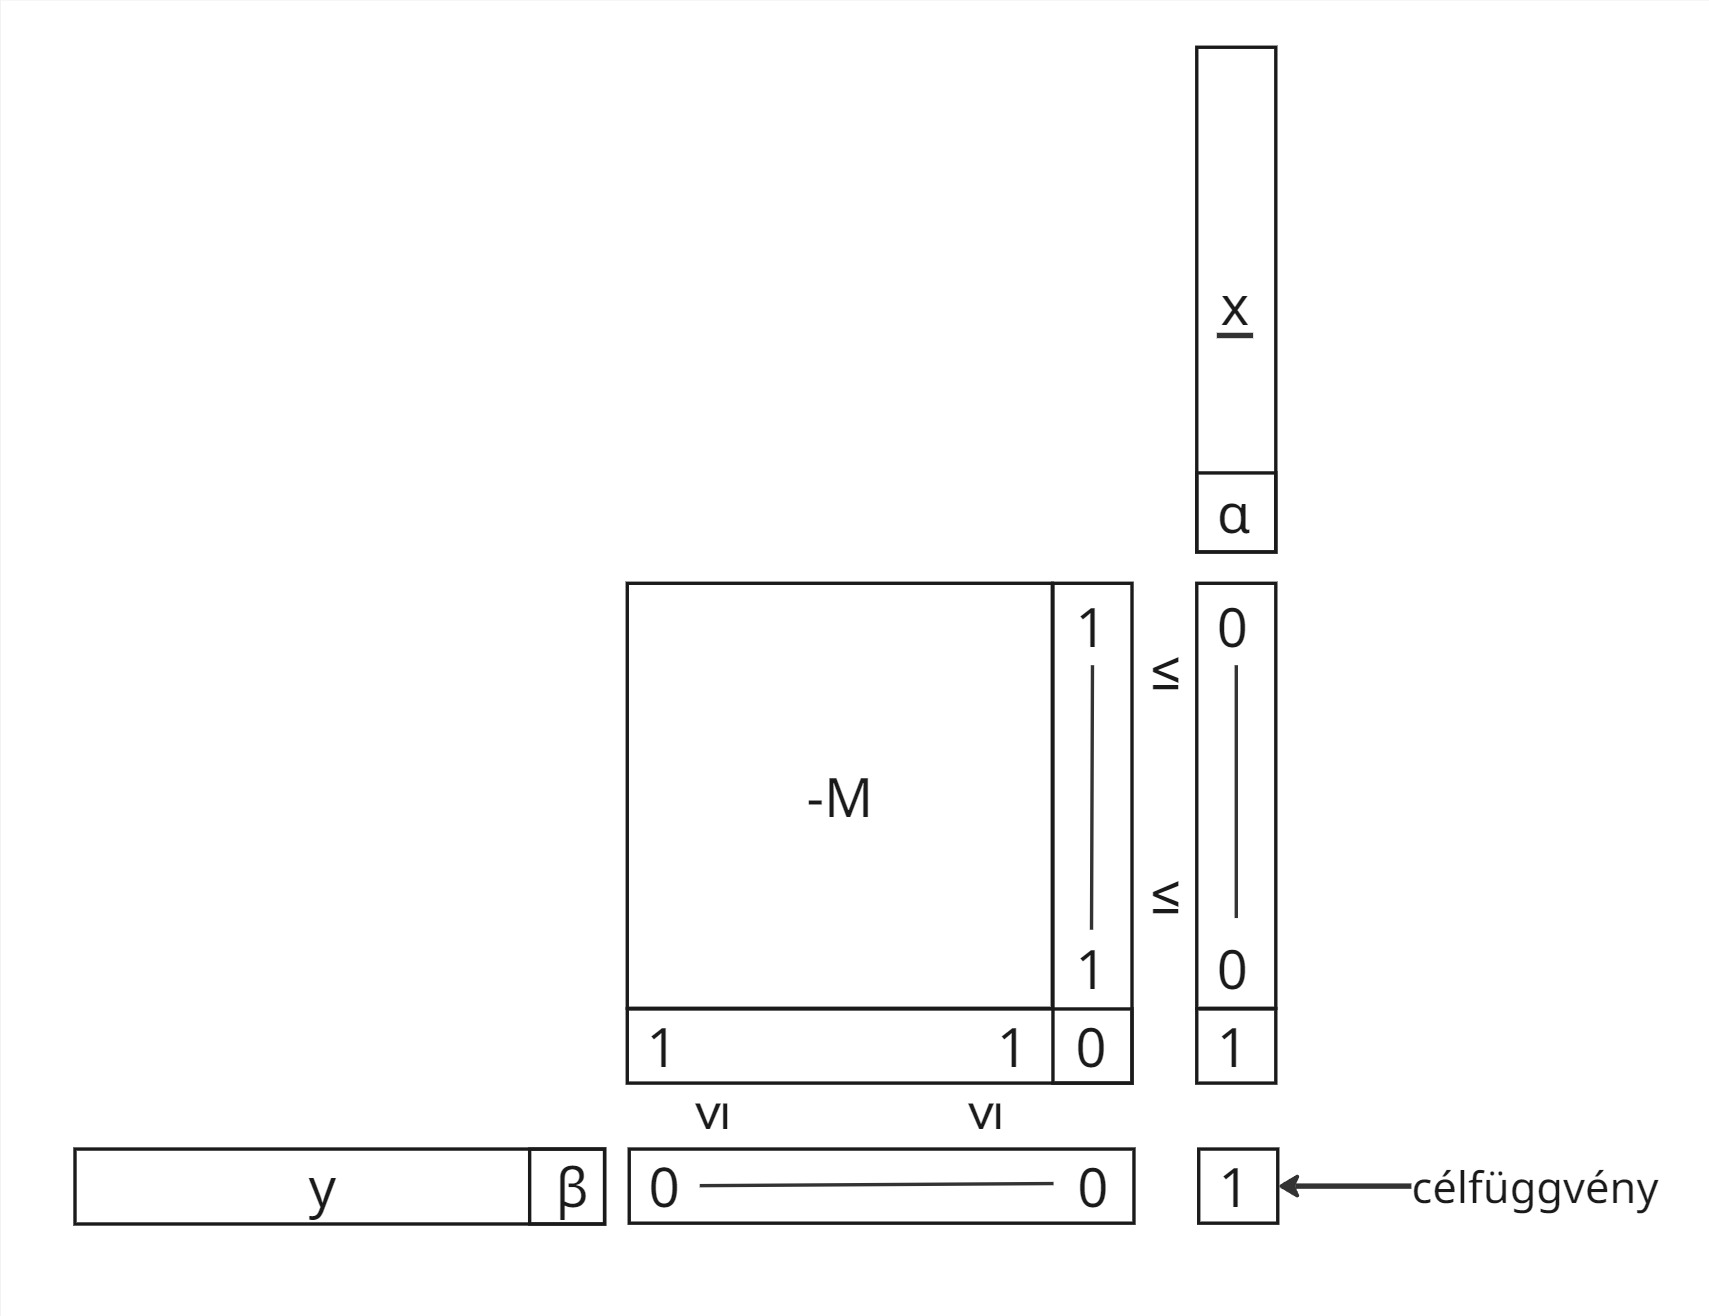
\includegraphics[width=100mm]{res/Neumann_tetel.jpg}
	%\end{center}
	
	Köv.: 2 személyes 0-összegű játék esetén a c maximin stratégiák kNE-t adnak 
	
	
	\begin{definition}{Csődprobléma}{}
		Adott egy $0 \leq E$ vagyon és n hitelező $0 \leq d_1 \leq ... \leq d_n$ követelésekkel úgy, hogy $E < \sum_i d_i$. Keressük a vagyon egy lehetséges szétosztását, vagyis olyan $x_1, ...m x_n$ kifizetéseket, amelyekre $0 \leq x_1, ..., x_n$ és $\sum_i x_i = E$ teljesülnek.
	\end{definition}
	
	\begin{definition}{Arányos szétosztás}{}
		A hitelezők a követeléseik arányában részesednek a vagyonból: $x_i = E \frac{d_i}{E_j d_j}$
	\end{definition}
	
	\begin{definition}{Egyenletes nyereségű szétosztás}{}
		Keressük azt a $\lambda$ nyereségértéket, amelyre ha a $\lambda$-nál kisebb követelésűek a saját követelésüket, a többiek pedig $\lambda$-t kapnak akkor éppen E lesz a kifizetések összege.
	\end{definition}
	
	\begin{definition}{Egyenletes veszteségű szétosztás}{}
		Keressük azt a $\mu$ veszteségértéket, amelyre ha a $\mu$-nél kisebb követelésűek semmit, a többiek pedig a követelésüknél $\mu$-vel kevesebbet kapnak, akkor éppen E lesz a
		kifizetések összege.
	\end{definition}
	
	\begin{definition}{Sorban állásos szétosztás}{}
		A hitelezőket egy meghatározott sorrendben szolgáljuk ki, az aktuálisan kiszolgált hitelező a még rendelkezésre álló vagyonból a követelése erejéig részesül.
	\end{definition}
	
	\begin{definition}{Kelmeszabály}{}
		Két hitelező között a kelmeszabály szerinti szétosztás a következőképpen történik: mindkét hitelező megkapja a saját követelésének a másik által nem követelt részét, a vitatott részen
		pedig fele-fele arányban osztoznak.
		\begin{center}
			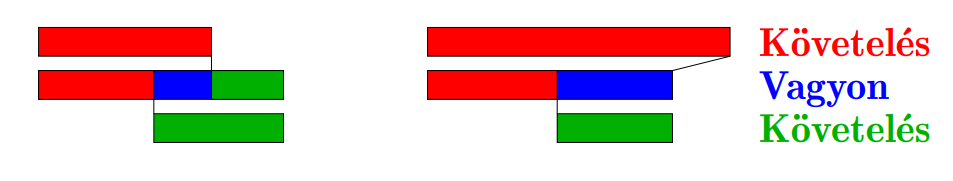
\includegraphics[width=150mm]{res/kelmeszabaly.png}
		\end{center}
		Ha van E-nél nagyobb követelés, azt E méretűként kezeljük.
	\end{definition}
	
	\begin{definition}{Kelmeszabály-konzisztens szétosztás}{}
		Egy $(x_1, ..., x_n)$ szétosztás kelmeszabály-konzisztens, ha
		bármely $i \neq j$ hitelezőpár a nekik összesen kiosztott $x_i + x_j$ vagyonból a $d_i$ és $d_j$ követeléseik alapján
		a kelmeszabály szerint éppen $x_i$ és $x_j$ részt kapna.
	\end{definition}
	
	\begin{definition}{Kaminski-féle közlekedőedény-rendszer}{}
		Tfh. mindkét hitelezőhöz tartozik egy-egy azonos keresztmetszetű, $d_1$ ill. $d_2$ térfogatú, hengeres tartály. Vágjuk félbe a tartályokat, kössük össze ezeket vékony csövekkel, és töltsük fel E (vagyonnagysággal) mennyiségű folyadékkal az így kapott közlekedőedény-rendszert. "Könnyen" látható, hogy folyadék épp a ksz szerint oszlik meg az egyes tartályokban. \\
		Így már nem nehéz ksz-konzisztens szétosztást találni: minden hitelezőhöz tartozzon egy-egy követelésnyi térfogatú tartály, kössük össze ezeket vékony csövekkel, és töltsük fel E mennyiségű folyadékkal a kapott rendszert.
		\begin{center}
			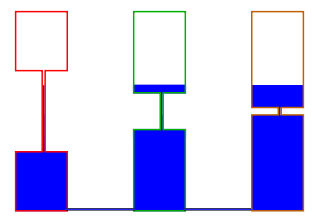
\includegraphics[width=100mm]{res/ksz_konzisztencia.png}
		\end{center}
	\end{definition}
	
	\begin{definition}{Öndualitás}{}
		Az összveszteség is ksz-konzisztensen van szétosztva.  
		A ksz-konzisztens szétosztás a csődjáték \textbf{nukleolusza}.  
		
		A nukleoluszt a \textbf{koalícióérték}, ill.\ a \textbf{többletvektor} definiálja.
	\end{definition}
	\paragraph{Példa}
	Legyen $E = 400$, $d_1 = 100$, $d_2 = 200$, $d_3 = 300$.  
	
	Egy koalíció értéke annyi, amennyi a többiek teljes kifizetése után marad:
	
	\[
	\begin{array}{c|cccccc}
		S      & \{1\} & \{2\} & \{3\} & \{1,2\} & \{2,3\} & \{1,3\} \\
		\hline
		v(S)   & 0     & 0     & 100   & 100     & 300     & 200
	\end{array}
	\]
	
	Egy $S$ koalíció \textbf{többlete} annyi, amennyit az értékén felül kap:
	\[
	e(x,S) = x(S) - v(S).
	\]
	
	\[
	\begin{array}{c|cccccc}
		\text{Koalíció} & \{1\} & \{2\} & \{3\} & \{1,2\} & \{2,3\} & \{1,3\} \\
		\hline
		v(S) & 0 & 0 & 100 & 100 & 300 & 200 \\
		x \text{ (arányos)} 
		& \frac{200}{3} & \frac{400}{3} & 200 & 200 & \frac{1000}{3} & \frac{800}{3} \\
		e(x,S) 
		& \frac{200}{3} & \frac{400}{3} & 100 & 100 & \frac{100}{3} & \frac{200}{3} \\
		y \text{ (ksz-konzisztens)} 
		& 50 & 125 & 225 & 175 & 350 & 275 \\
		e(y,S) 
		& 50 & 125 & 125 & 75 & 50 & 75
	\end{array}
	\]
	
	
	\begin{definition}{Többletvektor}
		A többletekből áll, növekvő sorrendben.
	\end{definition}
	\paragraph{Példa}\mbox{}\\
	$\Theta(x)$ = (33.3, 66.6, 66.6, 100, 100, 133.3) ill.\\
	$\Theta(y)$ = (50, 50, 75, 75, 125, 125) \\
	(a fenti táblázat alapján)
	
	\begin{definition}{Csődjáték nukleolusza}{}
		A nukleolusz az a szétosztás, ami lexikografikusan maximalizálja a többletvektort. Azaz: az első koordináta maximális, ezen belül a második koordináta is maximális stb.
	\end{definition}
	
	\begin{theorem}{Aumann-Maschler}{}
		A ksz-konzisztens szétosztás a csődjáték nukleolusza.
	\end{theorem}
	Biz.: *
	
	\newpage
	\section{Előadás}
	Osztozkodási játék, arányos szétosztást garantáló eljárások: oszt-választ, Fink, Tasnádi, Banach-Knaster, (diszkrét) mozgó késes, Even-Paz  (T 9.1, 9.2 (VKP 4.1))
	Irigységmentes szétosztások, Conway-Selfridge-eljárás.
	\begin{definition}{Osztozkodási probléma}{}
		A $[0,1)$ egy elosztása: \\
		$[0,1) = A_1 \cup A_2 \cup ... \cup A_n$, ahol $\forall A_i$ balról zárt, jobbról nyílt páronként diszjunkt intervallumok uniója, és $A_i$ véges sok.
	\end{definition}
	
	A játékosok $P_1, P_2, ..., P_n \quad P_i$ értékelő eloszlás fv.-e,\\
	 \[f_i:[0,1] \rightarrow [0,1], \text{ mon. növ.}
	 	\begin{cases} 
	 	f_i(0)=0 \\
	 	f_i(1)=1
	 	\end{cases} 	
	 \]

	$f_i(x):=[0,x)$ intervallum értéke a $P_i$ játékos számára.\\ 
	\\
	$P_i$ értékelő fv.-e $\mu_i$, ahol $I = [x,y)$ esetén $\mu_i(I) = f_i(y) - f_i(x)$. \\
	$\mu_i$ diszjunkt intervallumokon additív 
	
	\begin{definition}{Arányos elosztás}{}
		$(A_1, ..., A_n)$ arányos elosztások, ha $\mu_i(A_i) \geq (1/n) \quad \forall i $.
	\end{definition} 
	
	\begin{definition}{Mérés művelet}{}
		$Mér_i(x): f_i(x)$ érték meghatározása.
	\end{definition}
	
	\begin{definition}{Vágás művelet}{}
		$Vág_i(y): minf_i^{-1}(y)$ meghatározása.\\
		 (min. kell, mert nem szigorú $\rightarrow$ nem egyértelmű) \\
		$f(x) + [f(y)-f(x)]/2$.
	\end{definition}
	
	\begin{definition}{Oszt-választ protokoll}{}
		\begin{itemize}
			\item $P_1$ vág 1/2-nél 
			\item $P_2$ mér $P_1$ vágásánál
		\end{itemize}
	\end{definition}
	
	\begin{definition}{Fink eljárás}{}
		Egyesével érkező n db játékos
		\begin{itemize}
			\item $P_1$ megkapja az egészet
			\item Az i-dik lépésben $P_i$ megérkezik. Ekkor $P_1, ..., P_j,..., P_{i-1}$ már arányosan osztozkodott 
			\item $\forall$ játékos a saját részét i egyforma részre osztja szét
			\item $P_i \quad \forall$ játékostól választ 1-1 részt 
		\end{itemize}
	\end{definition}
	\begin{comment}
		
	\begin{tikzpicture}[
		node distance=18mm,
		every node/.style={draw, rectangle, rounded corners, align=center},
		arrow/.style={->, thick}
		]
		
		\node (start) {Bemenet:\\ követelések $d_i$, vagyon $E$};
		\node (init)  [below=of start] {Inicializálás:\\ $N_0=N$, $E_0=E$};
		\node (step)  [below=of init] {Egyenlő lépés\\ az aktív játékosokon};
		\node (check) [below=of step] {Vizsgálat:\\ $d_i=0$ vagy\\ $\sum d_i = E_k$?};
		\node (fix)   [below left=of check, xshift=-8mm] {Kifizetés rögzítése};
		\node (red)   [left=of step, xshift=8mm] {Redukció:\\ $N_{k+1},E_{k+1}$};
		\node (end)   [below=of check] {Megállás:\\ Fink-elosztás};
		
		\draw[arrow] (start) -- (init);
		\draw[arrow] (init) -- (step);
		\draw[arrow] (step) -- (check);
		\draw[arrow] (check) -- node[right]{igen} (fix);
		\draw[arrow] (fix) -- (red);
		\draw[arrow] (red) -- (step);
		\draw[arrow] (check) -- node[right]{nem} (end);
		
	\end{tikzpicture}
	\end{comment}
	
	\begin{definition}{Tasnádi rekurzív módszere}{}
		\begin{itemize}
			\item $P_1$ felosztja a $[0,1)$-t $n$ egyforma részre és mindegyikhez kibocsát $n-1$ jegyet
			\item Minden játékos ($P_2, ..., P_n$) a számára legjobb $n-1$ részhez húz 1-1 jegyet
			\item Ezek után mindenkinek $n-1$ jegye lesz
			\item Minden részt arányosan kiosztanak a jeggyel rendelkező játékosok között Tasnádi-eljárással
		\end{itemize}
	\end{definition}
	
	\begin{definition}{Diszkrét mozgó késes eljárás}{}
		\begin{itemize}
			\item $Vág_i(1/n) \quad \forall i $ [ábra]
			\item Aki legbalrább jelöl, az vág és távozik
			\item Ismételjük a maradék intervallumon, amíg el nem fogy
		\end{itemize}
		Művelet igény $n+(n-1)+(n-2)+...+1 =\binom{n+1}{2}$
	\end{definition}
	\href{https://youtu.be/GeEghYnuVps?si=soXOO_Iw5EsowTf3}{Videó}
	
	Ennek különböző verziói: Banach-Kraster, Dubins-Spanier
	
	\begin{definition}{Even-Paz protokoll (módosított)}{}
		
		\begin{itemize}
			\item $Vág(\lfloor n/2 \rfloor /n) \quad \forall i$ [ábra] 
			\item Az $\lfloor n/2 \rfloor$-dik jel mentén vágunk
			\item A bal oldali részt az $\lfloor n/2 \rfloor$ legkisebb jelet lerakó játékos, a jobb oldalit pedig az $\lceil n/2 \rceil$ legmagasabb jelet lerakó játékos közt osztjuk szét
			\item Így a baloldalon $\lfloor n/2 \rfloor$, a jobboldalon $\lceil n/2 \rceil$ játékos osztozik arányosan az Even-Paz eljárást követve
		\end{itemize}
		Művelet igény: $O(n\cdot logn)$ \\
	\end{definition}

	\begin{definition}{Irigységmentesség}{}
		$A_1, A_2, ..., A_n$ eloszlás irigységmentes, ha $\mu_i(A_i) \geq \mu_i(A_j) \quad \forall i\neq j$.
	\end{definition}
	
	\begin{observation}{}{}
		\begin{itemize}
			\item I.m. $\Rightarrow$ arányos
			\item Ha $A_1,...,A_n$ részek adottak és $P_1,P_2,...,P_n$ sorrendben választanak 1-1 részt $\Rightarrow$ csak később választó játékos lehet irigy korábban választóra
			\item $\mu_n(A_1) = \mu_n(A_2) = ... = \mu_n(A_n) \Rightarrow $ az utolsónak választó játékos nem lesz irigy 
		\end{itemize}
	\end{observation}
	
	\begin{definition}{Selfridge-Conway-eljárás}{}
		3 játékos: $A, B, C$. Cél: irigységmentes elosztás
		\begin{enumerate}
			\item $A$ 3 egyforma részre oszt
			\item $B$ preferenciája ezen részeken: x > y > z
			\item $B$ kettévágja x-et $x=x' \cup m$ úgy, hogy $\mu_B(x') = \mu_B(y)$
			\item $x', y, z$ darabokból választanak $C, B, A$ sorrendben úgy, hogy $B$ $x'$-t választja, ha tudja
			\item $P(x')$ az $x'$-t kapó játékos $P(x'), P(\overline{x'}) \in {C, B}, $
			\item $P(\overline{x'})$ $m$-et 3 egyforma részre osztja
			\item E 3 részt $P(x'), A, P(\overline{x})$ sorrendben osztják ki 
		\end{enumerate}
	\end{definition}
	\href{https://youtu.be/kaMKInkV7Vs?si=KuY9wgFSSZ5t7DBd}{Videó} \\
	Biz.: ppt
	
	\newpage
	\section{Előadás}
	Elosztás meghatározása szavazással, szavazási modell (alternatívák, szavazók, preferenciák, TVSZ és TVF), konkrét mechanizmusok (jóváhagyásos, többségi, Borda- és Copeland-szavazás) Condorcet-győztes. Mechanizmusok tulajdonságai (szimmetrikus, semleges, egyhangú, FLA, manipulálható, taktikázásbiztos, diktatórikus) és Arrow tétele. )T 6.1, 6.3, VKP 4.2) A Gibbard-Satterthwaite-tétel.
	
	\begin{definition}{Szavazási modell}{}
		Legyen $N={1, ..., n}$ a szavazók halmaza és $A = \{a_1, ..., 1_k\}$ az alternatívák halmaza. Az $i.$ szavazó szavazata az alternatívák egy lehetséges sorrendje (permutációja), az ehhez tartozó rendezési reláció jele a $\prec_i$. Az $n$ szavazó egy lehetséges választási profilja a $\Pi = (\prec_1, ..., \prec_n)$. A szavazási mechanizmus egy $F(\Pi)$ társadalmi választási szabályt (TVSZ) határoz meg, mely egy választási profilhoz hozzárendeli a szavazás eredményét, azaz az alternatíváknak a közös döntés szerinti sorrendjét. A nyerte alternatíva a TVSZ sorrendjében az első, az $f(\Pi)$ társadalmi választási függvény (TVF) ezt a nyertes alternatívát rendeli hozzá a $\Pi$-hez.
	\end{definition}
	
	\begin{definition}{Többségi szavazás}{}
		A többségi szavazás TVZS-e megszámolja, hogy egy adott alternatíva hányszor fordul elő első helyen a szavazatokban és az alternatívákat ezen előfordulási darabszám szerinti csökkenő sorrendbe teszi. Egyenlőség esetén az első szavazó szavazata dönt.
	\end{definition}
	
	\begin{definition}{Borda-szavazás}{}
		Az $i.$ szavazó $a \in A$ alternatívához rendelt Borda-pontszáma $B_i(a) = k - l$, ahol $l$ az $a$ alternatíva sorszáma az $i.$ szavazó sorrendjében. Az $a$ Borda-pontszáma $B(a)$, a szavazók Bordapontszámainak az összege. A Borda-szavazás TVSZ-e a Borda-pontszám szerinti csökkenő sorrendbe rendezi az alternatívákat. Egyenlőség esetén az első szavazó szavazata dönt.
	\end{definition}
	
	\begin{definition}{Condorcet-konzisztencia}{}
		Az $a$ alternatíva legyőz egy tőle különböző $b$ alternatívát, ha szigorúan több szavazó sorolta $a$-t a $b$ elé a sorrendjében. Az $a$ alternatíva Condorcet-győztes, ha legyőzött
		minden más alternatívát (ilyen nem mindig van). Egy szavazási mechanizmus Condorcet-konzisztens, ha a Condorcet-győztest választja nyertesnek, amennyiben az létezik.
	\end{definition}
	
	\begin{definition}{Copeland-szavazás}{}
		Az $a \in A$ alternatíva Copeland-pontszáma $C(a) = w(a) - l(a)$, ahol $w(a)$ jelöli azon alternatívák darabszámát, melyeket a legyőzött, $l(a)$ pedig azok darabszámát, melyek legyőzték $a$-t. A Copeland-szavazás TVSZ-e a Copeland-pontszám szerinti csökkenő sorrendbe rendezi
		az alternatívákat. Egyenlőség esetén az első szavazó szavazata dönt.
	\end{definition}
	
	\begin{theorem}{}{}
		A Copeland-szavazás Condorcet-konzisztens
	\end{theorem}
	
	\begin{observation}{Szavazási mechanizmusok tulajdonságai}{}
		\begin{itemize}
			\item \textbf{Szimmetrikus / anonim}: A TVSZ által adott eredmény nem változik, ha a szavazók tetszőleges permutáció szerint helyet cserélnek egymással.
			\item \textbf{Semleges / pártatlan}: A TVSZ által adott eredmény nem változik, ha a szavazók tetszőleges permutáció szerint átcímkézik az alternatívákat és az eredeti preferenciasorrendjük szerint
			szavaznak, de az alternatívák új címkéit írják a szavazólapra, a kapott eredményt pedig visszakódolják az eredeti címkézésre.
			\item \textbf{Egyhangú}: Ha $a, b \in A$ különböző alternatívákra minden szavazó a-t előrébb sorolja b-nél a
			szavazatában, akkor a TVSZ eredményében is a előrébb lesz mint b.
			\item \textbf{Független a lényegtelen alternatíváktól (FLA)}: Ha a szavazók úgy módosítják a szavazatukat, hogy egy adott alternatívahalmaz elemeinek az egymáshoz viszonyított sorrendje mindenkinél változatlan marad, akkor ugyanezen alternatívák egymáshoz viszonyított sorrendje a
			TVSZ eredményében sem változhat meg.
			\item \textbf{Taktikázásbiztos / nem manipulálható}: Egy szavazó nem tud úgy hazudni a saját preferenciasorrendjéről, hogy számára jobb alternatíva jöjjön ki nyertesként, mintha őszintén szavazott
			volna.
		\end{itemize}
	\end{observation}
	
	\begin{theorem}{Gibbard-Satterthwaite tétel}{}
		Ha van legalább 3 alternatíva, továbbá $f$ szürjektív (mindegyik
		alternatíva előáll nyertesként valamilyen $\Pi$-re) és taktikázásbiztos, akkor $f$ diktatórikus.
	\end{theorem}
	
	\begin{theorem}{Arrow tétel}{}
		Ha van legalább 3 alternatíva, továbbá $F$ egyhangú és független a lényegtelen alternatíváktól, akkor $F$ diktatórikus.
	\end{theorem}
	
	\newpage
	\section{Előadás}
	A Vickrey-árverés taktikázásbiztossága. (VKP 4.2, 4.3)
	A VCG-árverési mechanizmus taktikázásbiztossága. Veszteség- és szubvenciómentesség a Clarke-szabály használata esetén nemnegatív hasznosságok mellett.
	\begin{definition}{Árverési model}{}
		$N = \{1, 2, ..., n\}$ licitálók\\ 
		$A = \{a_1, ..., a_k\}$ alternatívák \\
		$\hat{v}_i: A \rightarrow \mathbb{R} \forall i \in N$ az i-dik licitáló értékelése \\
		$v_i: A \rightarrow \mathbb{R}$ az i-dik licitáló licitje \\
		$S_i:$ az i-dik licitáló lehetséges licitje\\
		$S = S_1 \times ... \times S_n$, S elemei a licitprofilok, $\underline{v} \in S \Rightarrow \underline{v} = (v_1, ... v_n)$
	\end{definition}
	
	%% $\underline{v} \in S \Rightarrow v = (v_1, ..., v_n)$
	%% ez nem tudom hova jön xd
	
	\begin{definition}{Árverési mechanizmus}{}
		$M = (f, p_1, ... p_n)$, ahol $f: S \rightarrow A$ a győztes alternatívát kiválasztó a fv. és $p_i: S \rightarrow \mathbb{R}$ mutatja meg, hogy az i-dik licitáló mennyit fizet az $f(\underline{v})$ alternatíva győzelme esetén
	\end{definition}
	
	Az i-dik licitáló nyeresége $u_i(\underline{v}) = \hat{v}_i (f(\underline{v}))-p_i(\underline{v})$
	
	\begin{definition}{M mechanizmus taktikázás biztos}{}
		Ha $u_i(\underline{v}) \leq u_i(v_{-i},\hat{v}_i) \quad \forall \underline{v} \in S \quad \forall i \in N$
	\end{definition}
	
	\begin{definition}{Vickrey-Clarke-Groves (VCG)}{}
		\begin{itemize}
			\item $f(\underline{v}) maximalizálja \sum_{i=1}^{n} v_i (a) \quad a\in A$-ra, azaz $\sum_{i=1}^{n} v_i (f(\underline{v})) \geq \sum_{i=1}^{n} v_i(a) \\ 
			\forall a \forall \underline{v} \in S$
			\item $p_i(\underline{v}) = h_i(\underline{v}_{-i}) - \sum_{j \neq i} v_j (f(\underline{v})) $ teljesül, ahol tetszőleges $h_i: S_{-i} \rightarrow \mathbb{R}$
			%% $\forall \underline(v) $\forall$ i$
			%% ezt se tudom hova jön
		\end{itemize}
	\end{definition}
	
	\begin{theorem}{}{}
		VCG taktikázás biztos $\forall h$-ra
	\end{theorem}
	 Biz.:
	 
	\begin{definition}{M szubvenciómentes}{}
		Ha $p_i \geq 0 \quad \forall i$
	\end{definition}
	
	\begin{definition}{M veszteségmentes}{}
		Ha $ \forall i \in N \quad \forall \underline{v} \in S \quad u_i(\underline{v}) \geq 0$, és $v_i = \hat{v}_i$
	\end{definition}
	
	\begin{definition}{Clarke-szabály}{}
		$h_i(\underline{v}_{-i}) = max\{ \sum_{i \neq j} v_j(a): a \in A\}$
	\end{definition}
	
	\begin{theorem}{}{}
		A VCG mechanizmus a Clarke-szabállyal veszteség- és szubvenció mentes, ha $\hat{v}_i(a) \geq 0 \quad \forall i \forall S$ 
	\end{theorem}
	Biz.:
	
	\newpage
	\section{Előadás}
	Újraosztási feladat, gyengén blokkoló koalíció, erős mag, felső körcsere (TTC) algoritmus. (VKP 4.3, 4.4) A TTC taktikázásbiztos tulajdonsága, piaci egyensúly és erős mag kapcsolata a lakáspiac esetén, piaci egyensúly keresése felső körcserével.
	\begin{remark}{Terminológia}{}
		Egyenértékűnek számít a jegyzetben a szendvics, jószág és a lakás.
	\end{remark}
	\begin{definition}{Újraosztási feladat}{}
		$N = \{1, 2, ..., n\} \preceq_i \in P = \{1, 2, ..., n\}$-en szigorú preferencia rendezések $\forall i \in N$ \\
		$\Pi = (\preceq_1, ..., \preceq_n) \in P^n$ preferencia profil \\
		$f: P^n \rightarrow S_N$ (= N.en a permutációk halmaza) mechanizmus, ahol $f(\Pi) = \sigma$ esetén $\sigma(i) = j$ jelenetése az, hogy i-dik játékos a j-dik játékos jószágát kapja meg
	\end{definition}
	
	\begin{definition}{Gyengén blokkolás}{}
		$\sigma \in S_N$-et a $B \subseteq N \quad$ gyengén blokkolja, ha $\exists \pi \in S_B$, amire a $\sigma(i) \prec_i \pi(i), \forall i \in B$ és $\exists j \in B :  \sigma(j) \preceq_j \pi(j) $\\
		$\sigma$ erős mag, ha $\nexists$ gyengén blokkoló koalíció. 
	\end{definition}
	
	\begin{definition}{}{}
		$S \subseteq N D(S)$ irányított segédgráf csúcsai: $S \forall i $ csúcsból 1-1 irányított él fut abba a csúcsba, amelyik lakását i a legjobban preferálja az S-beliek közül.
	\end{definition}
	
	\begin{definition}{Top Trading Cycles algoritmus}{}
		\begin{enumerate}
			\item $S_i = N \quad i = 1$
			\item $S_i = \emptyset \rightarrow $ END
			\item $S_i \neq \emptyset \quad N_i = C(D(S_i)) \quad S_{i+1} =  S_i\backslash N_i$
			\item $N_i$-beli játékosokra definiáljuk a $\sigma$-t a $D(S_i)$-beli élek mentén
			\item $i = i+1$ GOTO 2. lépés
		\end{enumerate}
	\end{definition}
	
	\begin{remark}{}{}
		Innentől $\sigma$ a TTC outputja
	\end{remark}
	
	Példa a működésre: \href{https://blockchain-academy.hs-mittweida.de/courses/game-theory-blockchain/lessons/cooperative-game-theory/topic/top-trading-cycle-algorithm/}{videó}
	
	\begin{theorem}{Lemma}{}
		Ha $S \neq \emptyset$ $\Rightarrow D(S)$ tartalmaz irányított kört %%[diszjunkt körök] %%
	\end{theorem}
	
	\begin{definition}{}{}
		$C(D(S))$ := D(S)-beli körök csúcshalmaza
	\end{definition}
	
	\begin{definition}{}{}
		j játékos rangja i, ha $j \in N_i$
	\end{definition}
	
	\begin{theorem}{Lemma}{}
		Ha j játékos egy újraosztás során $\sigma$-hoz képest jobban jár $\rightarrow$ a saját rangjánál kisebb rangú játékos lakását kapja \\
		Ha j a saját rangjánál nagyobb rangú játékos lakását kapja $\Rightarrow \sigma$-hoz képest rosszul
		
		
		 jár 
	\end{theorem}
	
	\begin{theorem}{Shapley-Scart-tétel}{}
		\begin{enumerate}
			\item a TTC $\sigma$ outputja benne van az erős magban
			\item másrészt nincs a $\sigma$-n kívül más eleme az erős magnak
		\end{enumerate}
	\end{theorem}
	Biz.: \\
	\url{https://www.sciencedirect.com/science/article/pii/S0304406824000296}
	
	\begin{definition}{}{}
		f újraosztási mechanizmus csoportosan manipulálható, ha $\exists M \subseteq N, \exists \pi \in P^N, \exists \pi_M \in P^{|M|} $\\
		$f(\pi)(j) \preceq_j f(\pi_M , \pi_{-M})(j) \forall j \in M$ és $\exists m \in M : f(\pi)(m)\prec_m f(\pi_M, \pi_{-M})$
	\end{definition}
	
	\begin{definition}{}{}
		f csoportosan tagadásbiztos, ha nem csoportosan manipulálható.
	\end{definition}
	
	\begin{theorem}{}{}
		TTC csoportosan tagadásbiztos
	\end{theorem}
	Biz*.: [előadáson nem fejeztük be]
	
	\begin{definition}{Piaci egyensúly}{}
		$p: N \rightarrow \mathbb{R}$ ár függvény és $\sigma \in S_N$ \\
		a $(p, \sigma)$ piaci egyensúly, ha
		\begin{itemize}
			\item $p (\sigma(i)) \preceq p(i) \quad \forall i$
			\item $\sigma(i) \preceq_i j \Rightarrow p(i) < p(j)$
		\end{itemize}
	\end{definition}
	
	\begin{statement}{}{}
		$(p, \sigma) PE \Rightarrow \sigma$ erős magbeli k.
	\end{statement}
	Biz.:
	
	\begin{observation}{}{}
		$\sigma$-beli cserekörök mentén a lakások árai nem változnak.
	\end{observation}
	
	\begin{statement}{}{}
		$\sigma$ a TTC outputja $\Rightarrow \exists p : N \rightarrow \mathbb{R}$, amire $(p, q)$ piaci egyensúly.
	\end{statement}
	Biz.: legyen $p(i) = |N|-r(i) \leftarrowtail$ i rangja [$|N|: játékosok száma$]
	
	\newpage
	\section{Előadás}
	Egyetemi felvételi probléma, visszavezetése stabil párosításra, keretszámot fel nem töltő szakok helyzete. Vonalhúzási probléma, stabil ponthatár keresése monoton operátorral. Ponthatárnövelő és -csökkentő algoritmus, szak- és jelentkező-optimális stabil ponthatár. Ponthatár és felvett hallgatók száma közti összefüggés.\\
	
	
	Láttuk: $M_1, M_2$ stabil párosítások G páros gráfban $\Rightarrow$ $V(M_1) = V(M_2)$
	
	\begin{theorem}{}{}
		A fiúk számára a lánykérő algoritmus taktikázás biztos \\
		\begin{center}
			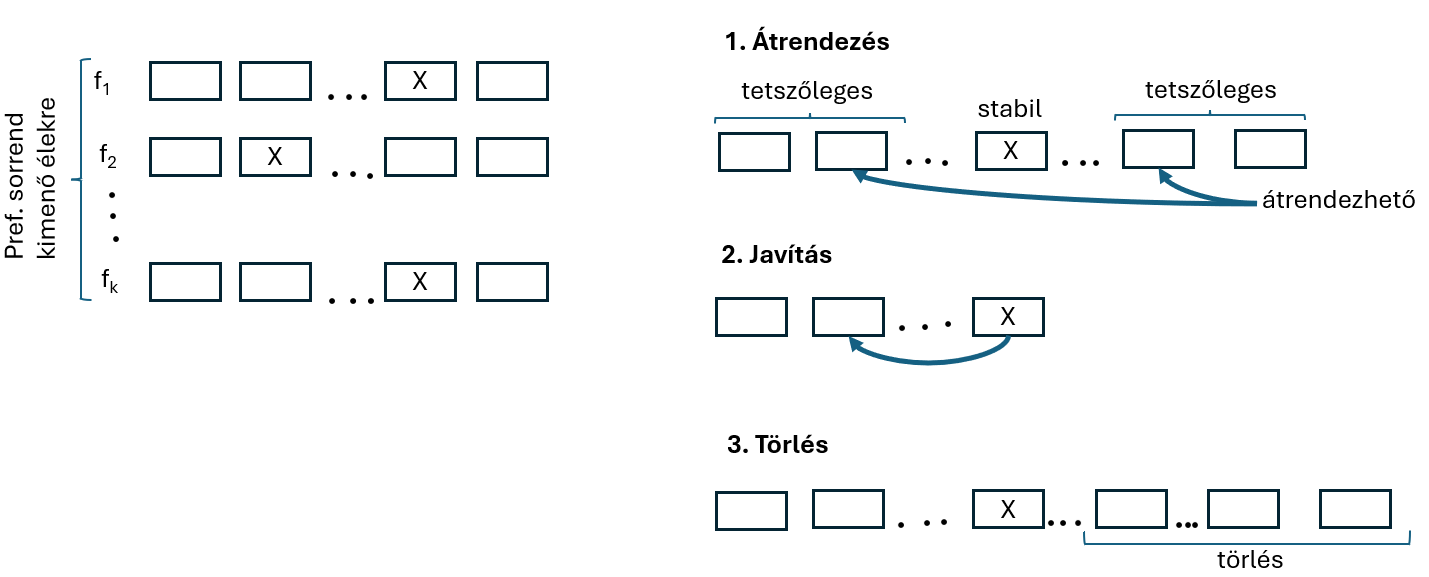
\includegraphics[width=150mm]{res/fiu_opt_parositas.png}
		\end{center}
	\end{theorem}
	
	\begin{observation}{}{}
		átrendezés, javítás, "törlés": megőrzik a konkrét stabil párosítást
	\end{observation}
	Biz.: 
	\begin{center}
		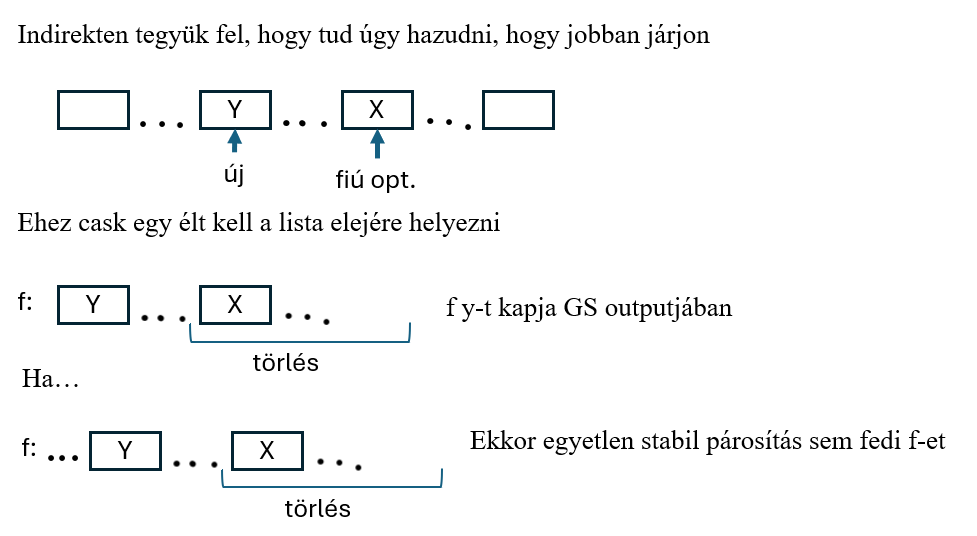
\includegraphics[width=150mm]{res/tabil_parositas_biz.png}
	\end{center}
	y-t mozgassuk előre $\Rightarrow$ előző eset, de itt f-et továbbra sem fogja stabil párosítás fedni.\\
	Ellentmondás: f ugyanúgy hazudott, de egyik esetben van stabil párja, a másikban nincs
	
	\begin{theorem}{TTC csoportosan taktikázás biztos}{}
		Tfh. $C_1, C_2, ...$ cserekörök jönnek létre az őszinte TTC-ben \\
		Hazug TTC cserekörei $C'_1, C'_2,...$ legyen $C'_i$ az első olyan csereköre ebben a sorrendben, ami nem jelenik meg  az őszinte TTC cserekörei között \\
		
		\begin{center}
			\begin{minipage}{0.45\textwidth}
				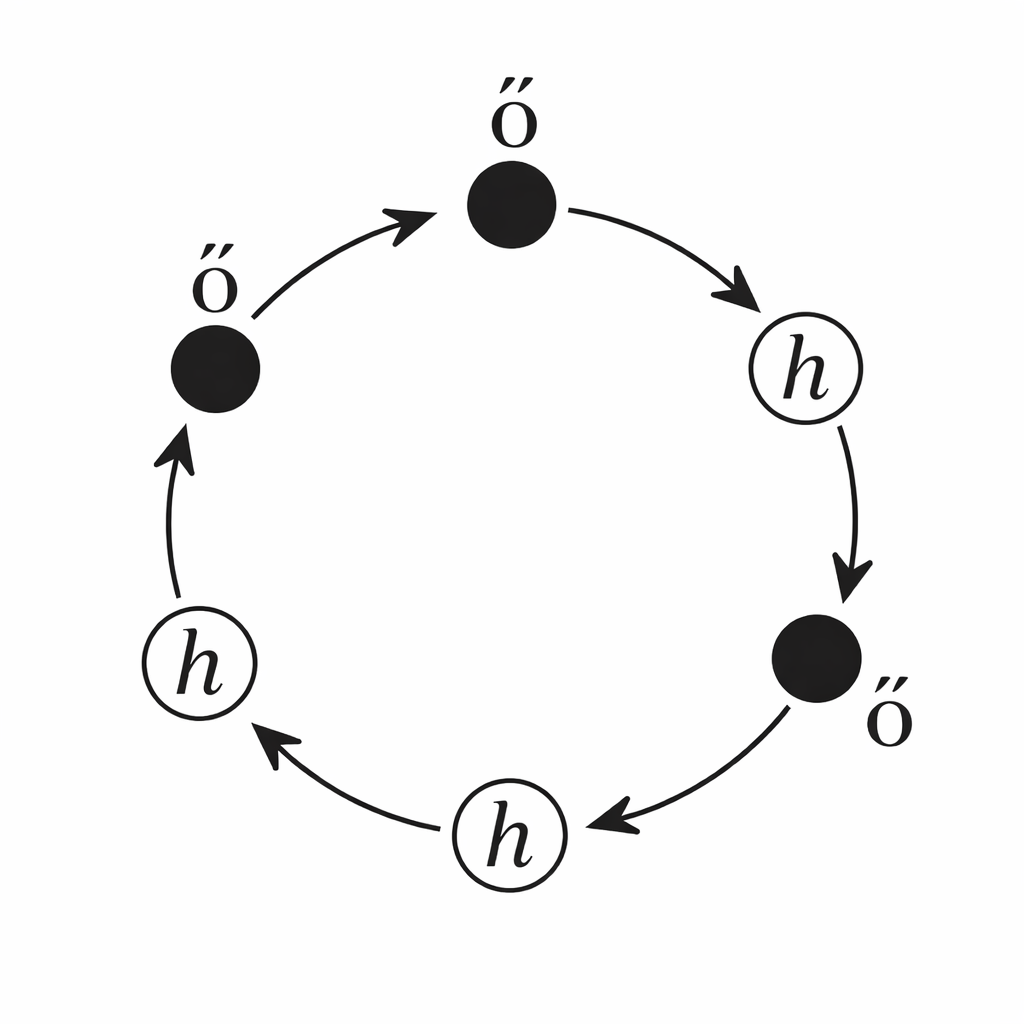
\includegraphics[width=\linewidth]{res/ttc_csop_takt_biz.png}
			\end{minipage}\hfill
			\begin{minipage}{0.45\textwidth}
				$C'_i$\\
				ő: őszinte\\
				h: hazug
			\end{minipage}
		\end{center}
		
		$C'_i$-ben kétféle lakás tulajdonos lehet \underline{őszinte} és \underline{hazug}. Őszinte játékos őszinte TTC szerinti cserekörében szereplő játékosok még a piacon vannak $\Rightarrow$ őszinte játékos nem jár rosszul $C'_i$-ben az őszinte TTC-hez képest. \\
		Tfh. egyetlen hazug játékos sem jár rosszul az őszinte TTC-hez képest. Legalább 1 játékos $C'_i$ másik lakást kap, mint az őszinte TTC szerint. Mivel senki sem jár rosszul $\rightarrow$ valaki jobban jár $\Rightarrow$ blokkoló koalíciót kapunk. \\
		Őszinte TTC output-ja magbeli $\Rightarrow$ $\nexists$ blokkoló koalíció $\Rightarrow$ ellentmondás!
		
	\end{theorem}
	
	\begin{definition}{Egyetemi felvételi probléma}{}
		Input: $G=(S \cup J, E)$ páros gráf, ahol 
		\begin{itemize}
			\item S: szakok
			\item J: jelentkezők
			\item E: jelentkezések
			\item $\forall s \in S$ szaknak van szigorúan preferált sorrendje a hozzá érkezett jelentkezésekben  
			\item $\forall j \in J$ jelentkező sorba rendezve
			\item $\forall s \in S$ szakhoz adott $q_s$ keretszám
		\end{itemize}
	\end{definition}
	
	\begin{definition}{Felvételi séma}{}
		$F \subseteq E$, amire $\forall j \in J$-ből $\leq 1$ F-beli él indul. $\forall s \in S$ szakból $\leq q_s$ él indul \\
		$e = j_s$ él blokkolja az F felvéltelek számát, ha
		\begin{itemize}
			\item j fedetlen vagy j-t egy e-nél rosszabb él fedi
			\item s nem töltötte fel a $q_s$ keretszámát vagy S-ből indul e-nél rosszabb él
		\end{itemize}
	\end{definition}
	
	\begin{statement}{}{}
		Felvételi séma stabil, ha $\nexists$ blokkoló él.
	\end{statement}
	
	\begin{statement}{}{}
		Egyetemi felvételi probléma visszavezethető páros gráf stabil párosításának keresésére
	\end{statement}
	Biz.: \\
	$S':=\{s_i: s \in S 1 \leq i\leq q_s\}$ \\
	$E':=\{j_{s_i}: j_S \in E 1 \leq i\leq q_s\}$ \\
	$\preceq_{s_i}: \preceq_s$-ből öröklődik \\
	$˛\preceq_j: j_{s_i} \preceq j_{sk}, ha j_s < j_s' ha s \ngeq s'$ és $i < k$, ha $s=s'$ \\
	$G'=(J \cup S',E')$
	
	\begin{statement}{M párosítás G'-ben}{}
		M vetülete G-ben felvételi séma, ahol M vetülete $P(M)={j_s : \exists i j_{s_i} \in M}$ \\
		$P(M) \forall j \in J$-ből $\leq 1$ élt, $\forall s \in S$-ből legfeljebb $q_s$ élt tart
	\end{statement}
	
	\begin{statement}{}{}
		M G' stabil párosítás $\Leftrightarrow$ P(M) stabil felvételi séma
	\end{statement}
	Biz.: 
	Tfh: M stabil párosítás G'-ben. P(M)-nél láttuk, hogy felvételi séma \\
	Tfh. $j_s$ él blokkolja P(M)-et $\Rightarrow$ s (1) vagy nem tölttöte fel $q_s$-t vagy (2) felvett j-nél rosszabb jelentkezőt \\
	(1) $s_i$ fedetlen, $j_{s_i}$ blokkol M-ben  \\
	(2) $s_i$ blokkolja M-et \\
	Tfh.: F stabil felvételi séma $\rightarrow$ cél: $\exists G'$-ben olyan M stabil párosítás, amin P(M)=F\\
	M' konstukciója: az s szak által felvett jelentkezőket az s preferenciája szerint ültetjük az 1., 2., ... stb. helyekre. Könnyen látható, hogy M stabil párosítás G-ben.
	\\
	
	Következmény: J jelentkező-optimális, szak-optimális stabil felvételi séma \\
	$\forall$ 2 stabil felvételi sémában ugyanazok a jelentkezők lesznek felvéve és $\forall$ szak ugyanannyi jelentkezőt vesz fel a 2 sémában
	
	\begin{definition}{Vonalhúzási probléma}{}
		$S,J,E \quad \forall j \in J \prec_j \quad \forall j_s \in E \quad r_{j_s}$ pontszám \\
		ponthatár: $l: S \rightarrow N$ rögzített $l$ mellett, $j_s \in E \quad \underline{eredményes} : r_{j_s} \geq l(s) \quad $, $ \underline{sikeres}$: (1) eredményes (2) j számára nincs ennél jobb eredményes jelentkezés \\
		$l \quad \underline{megengedett}$, ha F(l) felvételi séma \\
		$l \quad \underline{kritikus}$, ha $\forall s \in S$ igaz, hogy vagy $l(s) = 0$ vagy $l(s)$-et 1-gyel csökkentjük és a többi $l(s')$ változatlan maradna $\Rightarrow$ az így kapott ponthatár már nem volna megengedett. \\
		$l \quad \underline{stabil}$, ha megengedett és kritikus
	\end{definition}
	
	\begin{definition}{Ponthatárcsökkentő algoritmus}{}
		Tfh.: $r_{j_s} \leq 500$ \\
		$l = 500 \quad \varphi(l) = l'$, ahol $l'(s)$-t úgy határozzuk meg, hogy a legkisebb olyan pontszám legyen, amire s még nem tölti túl a keretszámát, akkor, ha $\forall$ más szak ponthatára az l által meghatározott ponthatár. \\
		$500 \geq \varphi(500) \geq \varphi(\varphi(500)) \geq ... \Rightarrow \exists i : \varphi^{(i)}(500) = \varphi^{(i+1)}(500) \geq l \rightarrow$ stabil \\
		$\Rightarrow$ szak optimális felvételi séma \\
		$0 \leq \varphi(0) \leq \varphi(\varphi(0)) \leq ... \Rightarrow$ jelentkező optimális séma
	\end{definition}
	
	\newpage
	\section{Előadás}
	Népszerű párosítások, stabil párosítások népszerűsége, maximális élszámú népszerű párosítás keresése Kavitha algoritmusával.
	
	\newpage
	\section{Források}
	\begin{itemize}
		\item Dr. Fleiner Tamás és Nemkin Viktória előadásán elhangzottak
		\item A \url{https://www.cs.bme.hu/alje/} oldalon elérhető anyagok
		\item \href{https://www.cs.bme.hu/\%7Efleiner/alje2024/tematika.pdf}{Algoritmikus játékelmélet szóbeli tematika 2024}
		\item \href{https://www.cs.bme.hu/%7Efleiner/alje2025/tematika.pdf}{Algoritmikus játékelmélet szóbeli tematika 2025}
		\item \href{https://cs.bme.hu/~nemkin/jatek/}{Nemkin Viktória feladat megoldások}
		\item \href{http://tkiraly.web.elte.hu/students/jatekelmelet_jegyzet.pdf}{Végh László, Király Tamás, Pap Júlia: Játékelmélet jegyzet}
		\item \href{http://www.maths.lse.ac.uk/personal/stengel/lectnotes1-7.pdf}{Bernhard von Stengel: Game Theory Basics}   
	\end{itemize}
	
\end{document}
